%%%%%%%%%%%%%%%%%%%%%%%%%%%%%%%%%%%%%%%%%%%%%%%%%%%%%%%%%%%%%%%%%%%%%%%%%%%%%%%%%%%%%
%																					%
%	TRABAJO: Proyecto Integrador													%
%																					%
%		Titulo: 	Desarrollo de IP cores con procesamiento de Redes de Petri 		%
%					Temporales para sistemas multicore en FPGA						%
%																					%
%		Autores:	Juli�n Nonino													%
%					Carlos Renzo Pisetta											%
%		Director:	Orlando Micolini												%
%																					%
%	Parte: Resultados y Conclusiones												%
%	Capitulo: Resultados Obtenidos													%	
%	Archivo: chap_resultados.tex													%
%																					%
%%%%%%%%%%%%%%%%%%%%%%%%%%%%%%%%%%%%%%%%%%%%%%%%%%%%%%%%%%%%%%%%%%%%%%%%%%%%%%%%%%%%%

% Path Imagenes: ./desarrollo/resultados_conclusiones/resultados/img
% Nombre predeterminado imagenes: resultadosxx
%	xx es el numero de imagen

\lstset
{	language=C,               		% the language of the code
	basicstyle=\footnotesize,       % the size of the fonts that are used for the code
	numbers=left,                   % where to put the line-numbers
	numberstyle=\tiny\color{gray},  % the style that is used for the line-numbers
	stepnumber=1,                   % the step between two line-numbers. If it's 1, each line 
                       				% will be numbered
	numbersep=5pt,                  % how far the line-numbers are from the code
	backgroundcolor=\color{white},  % choose the background color. You must add \usepackage{color}
	showspaces=false,               % show spaces adding particular underscores
	showstringspaces=false,         % underline spaces within strings
	showtabs=false,                 % show tabs within strings adding particular underscores
	frame=none,                 	% adds a frame around the code
	rulecolor=\color{white},        % if not set, the frame-color may be changed on line-breaks within not-black text (e.g. comments (green here))
	tabsize=2,                      % sets default tabsize to 2 spaces
	captionpos=b,                   % sets the caption-position to bottom
	breaklines=true,                % sets automatic line breaking
	breakatwhitespace=false,        % sets if automatic breaks should only happen at whitespace
	%title=\lstname,                % show the filename of files included with \lstinputlisting;
		                            % also try caption instead of title
	keywordstyle=\color{violeta},      % keyword style
  	commentstyle=\color{dkgreen},   % comment style
  	stringstyle=\color{blue},      % string literal style
  	escapeinside={\%*}{*)},         % if you want to add LaTeX within your code
  	morekeywords={*,...},           % if you want to add more keywords to the set
  	deletekeywords={...}            % if you want to delete keywords from the given language
}

\chapter{Resultados Obtenidos}
	\label{chap:chap_resultados}

	En �ste cap�tulo se realizar� una descripci�n de los resultados obtenidos luego del desarrollo
	del \textbf{\emph{Procesador de Redes de Petri Temporales}}
	
	Dado que los IP cores desarrollados son totalmente parametrizables, en la primera secci�n del cap�tulo
	se realizar� un an�lisis del crecimiento de este IP core ante la variaci�n de los par�metros. Esto se 
	debe a que en las FPGA, el �rea es un factor muy importante.
	
	Luego, se realizar� una comparaci�n entre la resoluci�n de problemas con el procesador de Redes de Petri
	y la resoluci�n utilizando sem�foros. Esto se har� con el objetivo de comparar el mecanismo de 
	sincronizaci�n desarrollado con los existentes en la actualidad. Para esto, se realizar�n dos 
	pruebas, una con el problema \emph{Escritor/Escritor} que requiere un alto grado de sincronizaci�n, y otra
	con el problema de la \emph{F�brica de Mesas} y el de la \emph{Cena de los Fil�sofos} para probar las 
	restricciones temporales y las interrupciones.
	Los tres problemas ser�n implementados en el lenguaje \emph{C} y correr�n sobre el sistema operativo
	\emph{Xilinx Xilkernel} \cite{xilinx_xilkernel}.
		 
	% Crecimiento del tama�o del IP core
		%%%%%%%%%%%%%%%%%%%%%%%%%%%%%%%%%%%%%%%%%%%%%%%%%%%%%%%%%%%%%%%%%%%%%%%%%%%%%%%%
%	TRABAJO: Proyecto Integrador
%		Titulo: 	Desarrollo de IP cores con procesamiento de Redes de Petri 	
%					Temporales para sistemas multicore en FPGA					
%		Autores:	Juli�n Nonino												%					Carlos Renzo Pisetta										%		Director:	Orlando Micolini											
%%%%%%%%%%%%%%%%%%%%%%%%%%%%%%%%%%%%%%%%%%%%%%%%%%%%%%%%%%%%%%%%%%%%%%%%%%%%%%%%

% Path im�genes: ./resultados_conclusiones/resultados/img
% Nombre predeterminado im�genes: resultadosxx
%	xx es el numero de imagen

\section{Crecimiento del tama�o del IP core}
	\label{sec:crecimiento_ip_core}
	
	El IP core del procesador de Redes de Petri, es parametrizable seg�n la cantidad de plazas, transiciones y, del tama�o de cada elemento de datos usado. Considerando como \emph{p} al n�mero de plazas y \emph{t} al n�mero de transiciones, cada uno de los elementos que definen a la Red de Petri tienen el siguiente tama�o.
	
	\newpage
	
	\begin{figure}[H]
		\centering
		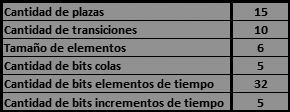
\includegraphics[width=0.4\linewidth,keepaspectratio]{./resultados_conclusiones/resultados/img/resultados01}
		\caption{Par�metros para analizar el crecimiento de los datos en redes de Petri con Tiempo}
		\label{fig:resultados01}
	\end{figure}
		
	Se utilizan estos valores para mostrar porque son los correspondientes a los IP cores generados para realizar las pruebas.	
	\begin{figure}[H]
		\centering
		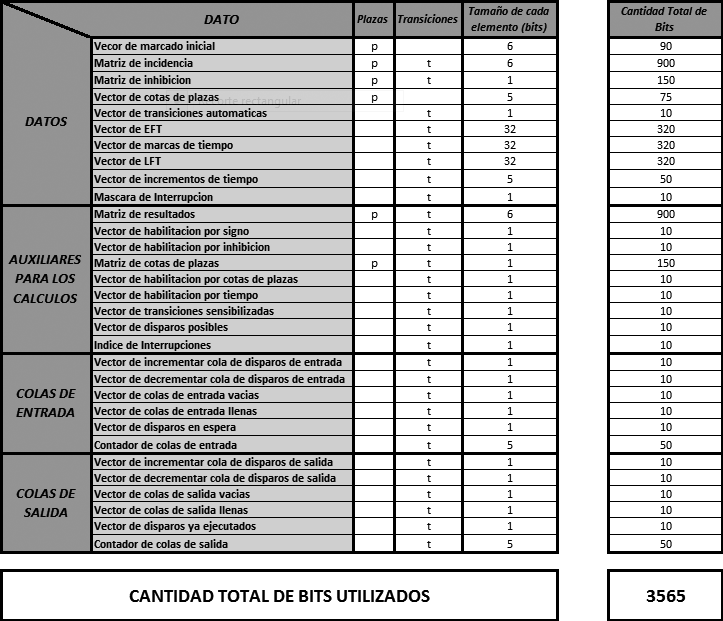
\includegraphics[width=1\linewidth,keepaspectratio]{./resultados_conclusiones/resultados/img/resultados02}
		\caption{Crecimiento de los datos dentro del IP core para Redes de Petri con Tiempo}
		\label{fig:resultados02}
	\end{figure}
	
	Los valores de la tabla anterior, representan la dependencia de cada uno de los datos internos del IP core con respecto a los par�metros de mismo, como cantidad de plazas, cantidad de transiciones, cantidad de bits de cada elemento, etc�tera. Por ejemplo, en el caso de la matriz de incidencia, se ve que var�a su tama�o seg�n la cantidad de plazas, en �ste caso 15, seg�n la cantidad de transiciones, para la Figura su valor es 10 y seg�n la cantidad de bits de cada elemento, en �ste caso, 6. Con estos valores, al ser una matriz, tiene $p�t$ elementos ($15�10=150$). Dado que cada elemento tiene 6 bits, la cantidad total de bits de la matriz de incidencia ser� $p�t�bits elementos$ ($150�6=900$)
	
	\begin{figure}[H]
		\centering
		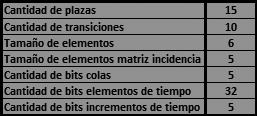
\includegraphics[width=0.4\linewidth,keepaspectratio]{./resultados_conclusiones/resultados/img/resultados03}
		\caption{Valores utilizados como par�metros para analizar el crecimiento de los datos en Redes de Petri Temporizadas}
		\label{fig:resultados03}
	\end{figure}
	
	\begin{figure}[H]
		\centering
		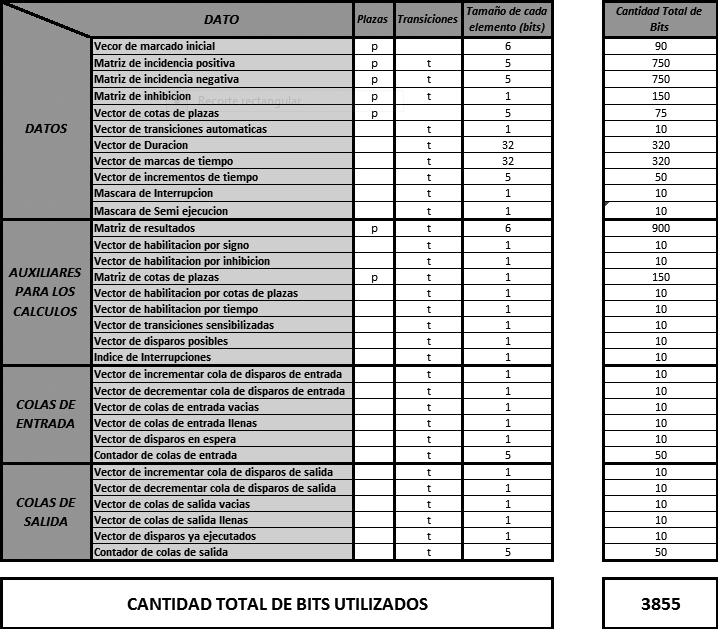
\includegraphics[width=1\linewidth,keepaspectratio]{./resultados_conclusiones/resultados/img/resultados04}
		\caption{Crecimiento de los datos dentro del IP core para Redes de Petri Temporizadas}
		\label{fig:resultados04}
	\end{figure}

	En base a estos datos, se ha sintetizado el sistema que incluye un procesador \emph{MicroBlaze} \cite{xilinx_microblaze} y el IP core del procesador de Redes de Petri variando los par�metros de este �ltimo como por ejemplo, cantidad de plazas, tama�o en bits de los elementos, etc�tera. Todas las mediciones que se mostrar�n han sido realizadas con el IP core para procesamiento de \emph{Redes de Petri con Tiempo}. 
	\\
	
	En �ste momento, en el Laboratorio de Arquitecturas de Computadoras (LAC), se dispone de dos kits de desarrollo con FPGA que son �tiles para este trabajo, el kit de Digilent Atlys \footnote{\url{http://www.digilentinc.com/Products/Detail.cfm?NavPath=2,400,836&Prod=ATLYS}} y, el kit llamado Zedboard \footnote{\url{http://www.digilentinc.com/Products/Detail.cfm?NavPath=2,400,1028&Prod=ZEDBOARD}} distribuido para fines acad�micos tambi�n por \emph{Digilent}. Como el kit de desarrollo \emph{Digilent Atlys} era el �nico disponible en el laboratorio al comenzar este trabajo, el proyecto del sistema fue generado para esta plataforma. se realiz� una medici�n del �rea de la FPGA ocupada para diferentes valores de los antes mencionados par�metros del procesador de Redes de Petri. Estas mediciones, han sido realizadas debido a que el �rea que ocupa un hardware dentro de un chip es un factor muy importante al momento de dise�ar e implementar circuitos integrados, mientras mayor sea el �rea del chip, mayor sera el costo del mismo \cite{hennessypatterson}. Los datos a medir fueron, cantidad de Flip-Flops utilizados, ya que se comprob� que cada bit necesario para la implementaci�n requiere un Flip-Flop para ser almacenado y cantidad de celdas l�gicas de la FPGA consumidas por la implementaci�n.

	\begin{figure}[H]
		\centering
		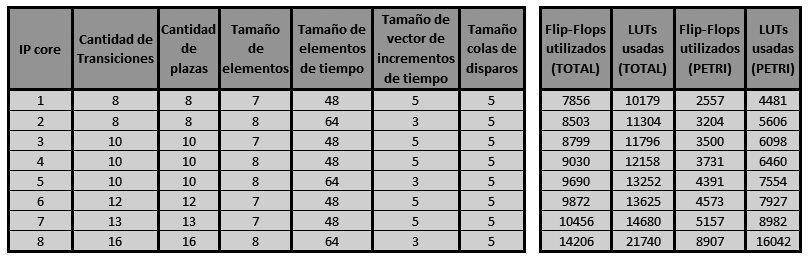
\includegraphics[width=1\linewidth,keepaspectratio]{./resultados_conclusiones/resultados/img/resultados05}
		\caption{Diferentes implementaciones del procesador de Redes de Petri en el kit Digilent Atlys (Tabla)}
		\label{fig:resultados05}
	\end{figure}

	Con los datos obtenidos (Figura \ref{fig:resultados05} y Figura \ref{fig:resultados06}), se pudo observar que una Red de Petri de gran tama�o no podr�a ser implementada en el kit Atlys, esto se debe a las siguientes razones. La cantidad de Flip-Flops y celdas l�gicas utilizadas por el procesador de Redes de Petri crece considerablemente. Como el kit de desarrollo no cuenta con un procesador propio, el \emph{MicroBlaze} con todos sus perif�ricos debe ser implementado en la FGPA. Por esta raz�n, el procesador de Redes de Petri tiene limitadas sus posibilidades de crecimiento debido al �rea ocupada por el resto de los componentes del sistema.

	\begin{figure}[H]
		\centering
		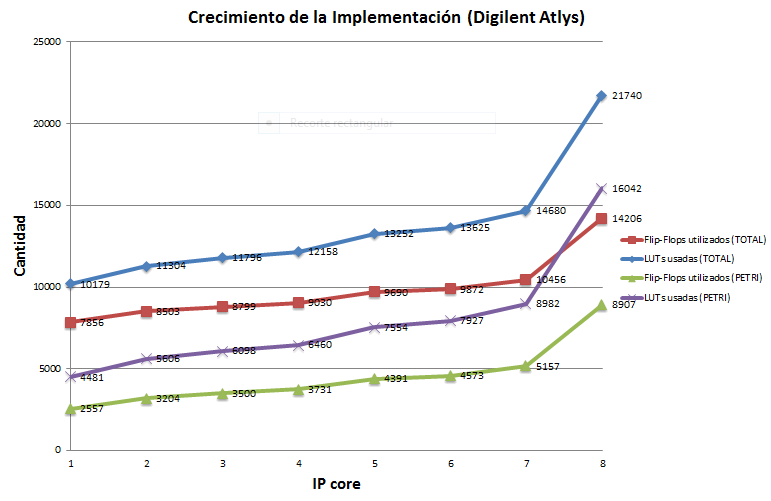
\includegraphics[width=1\linewidth,keepaspectratio]{./resultados_conclusiones/resultados/img/resultados06}
		\caption{Diferentes implementaciones del procesador de Redes de Petri en el kit Digilent Atlys (Gr�fica)}
		\label{fig:resultados06}
	\end{figure}
	Por las limitaciones enunciadas anteriormente, se han realizado mediciones similares para el kit de desarrollo ZedBoard. A pesar de no haber contado con �ste kit para el desarrollo del proyecto, actualmente en el Laboratorio de Arquitectura de Computadoras se cuenta con uno de ellos y uno de los trabajos en desarrollo es implementar los IP cores desarrollados a �ste nuevo kit. Una FPGA de mayor tama�o y un procesador dual core ARM A9 son algunas de las ventajas de este kit de desarrollo.
	\begin{figure}[H]
		\centering
		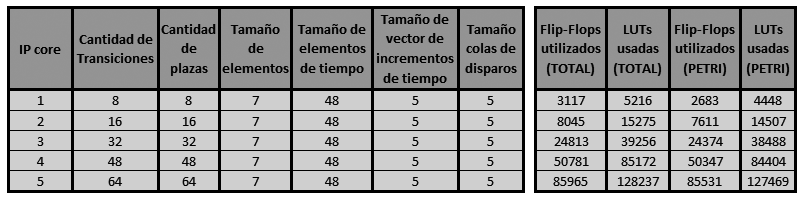
\includegraphics[width=1\linewidth,keepaspectratio]{./resultados_conclusiones/resultados/img/resultados07}
		\caption{Diferentes implementaciones del procesador de Redes de Petri en el kit Zedboard (Tabla)}
		\label{fig:resultados07}
	\end{figure}
	\newpage
	\begin{figure}[H]
		\centering
		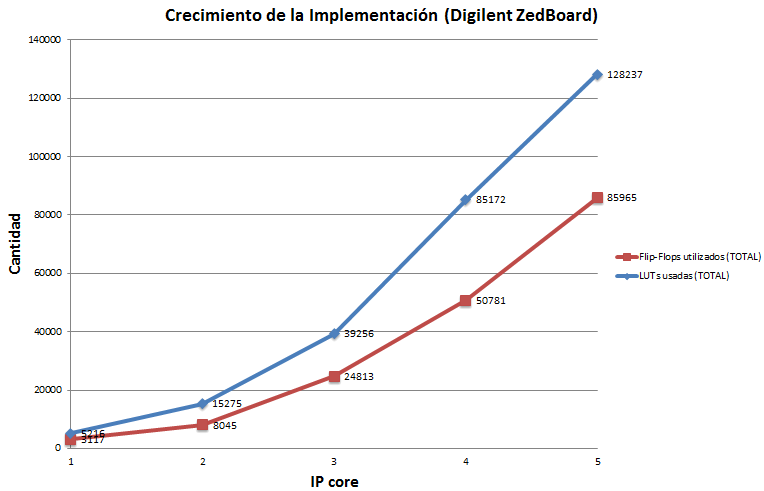
\includegraphics[width=0.9\linewidth,keepaspectratio]{./resultados_conclusiones/resultados/img/resultados08}
		\caption{Diferentes implementaciones del procesador de Redes de Petri en el kit Zedboard (Gr�fica Total)}
		\label{fig:resultados08}
	\end{figure}
	\begin{figure}[H]
		\centering
		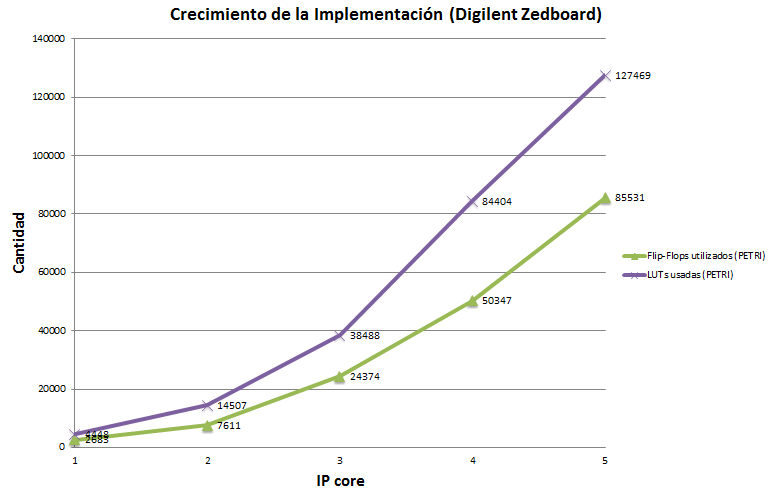
\includegraphics[width=0.9\linewidth,keepaspectratio]{./resultados_conclusiones/resultados/img/resultados09}
		\caption{Diferentes implementaciones del procesador de Redes de Petri en el kit Zedboard (Gr�fica Petri)}
		\label{fig:resultados09}
	\end{figure}
	\newpage
	El kit de desarrollo ZedBoard seg�n sus especificaciones cuenta con una FPGA con 106400 Flip-Flops y 85000 celdas l�gicas. En las gr�ficas de las Figuras \ref{fig:resultados08} y \ref{fig:resultados09} se observa como, en el caso de utilizar este kit de desarrollo podr�a implementarse un procesador de Redes de Petri de mas de 48 plazas por 48 transiciones brindando una mayor flexibilidad para modelar sistemas.
	
	Los datos obtenidos de la s�ntesis del IP core para este kit de desarrollo, son presentados en dos gr�ficas porque al utilizar solo una las curvas se superpon�an.
		
	Para ambos kits de desarrollo, se presentan las mediciones de Flip-Flops y LUTs del sistema total y tambi�n, los valores obtenidos s�lo para el IP core. Esto se realiz� para tener una idea del qu� parte de la FPGA era utilizada por el procesador de Redes de Petri y qu� parte por componentes anexos.
	
		
	% Medidas de rendimiento
		%%%%%%%%%%%%%%%%%%%%%%%%%%%%%%%%%%%%%%%%%%%%%%%%%%%%%%%%%%%%%%%%%%%%%%%%%%%%%%%%
%	TRABAJO: Proyecto Integrador
%		Titulo: 	Desarrollo de IP cores con procesamiento de Redes de Petri 	
%					Temporales para sistemas multicore en FPGA					
%		Autores:	Juli�n Nonino												%					Carlos Renzo Pisetta										%		Director:	Orlando Micolini											
%%%%%%%%%%%%%%%%%%%%%%%%%%%%%%%%%%%%%%%%%%%%%%%%%%%%%%%%%%%%%%%%%%%%%%%%%%%%%%%%

% Path im�genes: ./resultado_conclusiones/resultados/img
% Nombre predeterminado im�genes: resultadosxx
%	xx es el numero de imagen

\section{Medidas de rendimiento}
	\label{sec:medidas_rendimiento}
	
	En este trabajo, se ha desarrollado una nueva forma de modelar e implementar sistemas concurrentes, esto quiere decir que servir� como mecanismo de sincronizaci�n entre los diferentes procesos del sistema. Por esta raz�n, se desea determinar si el procesador de Redes de Petri presenta un mejor desempe�o frente a otros mecanismos de sincronizaci�n. En este caso se utilizar�n sem�foros para la comparaci�n debido a que es un mecanismo m�s liviano y sencillo que, por ejemplo, los monitores.
	\\
	
	Para calcular el rendimiento de la implementaci�n de un sistema con un procesador de Redes de Petri, se medir� la cantidad de pulsos de reloj necesarios para procesar los disparos y obtener la respuesta que permita sincronizar diferentes programas. Estas mediciones tambi�n se har�n sobre el mismo problema pero resuelto con sem�foros. Para realizar �stas mediciones, se utilizar� un IP core de Xilinx llamado AXI TIMER \cite{xilinx_axi_timer}. Es IP core, recibe una se�al indicando que debe comenzar a contar y cuenta a la velocidad del reloj del sistema. En cualquier momento, este timer puede ser detenido dando as� un valor que representa la cantidad de ciclos desde que se inicio hasta que se detuvo el contador. Si se desea obtener un valor en segundos, solo se debe dividir el valor entregado por el timer con la frecuencia del reloj del sistema.
	\\
	
	Una vez obtenidos los valores de tiempo para cada aplicaci�n, definiremos el rendimiento del uso del procesador de Redes de Petri de la siguiente manera:
	
	\begin{equation}
		\eta = \frac{S_{Sem}}{S_{Petri}}
		\label{eq:rendimiento}
	\end{equation}
	
	Donde,
		\begin{itemize}
		  	\item \textbf{\emph{$S_{Petri}$}} Tiempo de sincronizaci�n m�nimo utilizando el procesador de Redes de Petri. Tiempo que le toma a un proceso solicitar un disparo para obtener un recurso, obtenerlo y emitir el disparo para liberarlo.
	  		\item \textbf{\emph{$S_{Sem}$}} Tiempo de sincronizaci�n m�nimo utilizando Sem�foros. Tiempo que le toma a un proceso hacer la operaci�n \emph{wait} sobre un sem�foro para obtener un recurso, obtenerlo y hacer la operaci�n \emph{signal} sobre el sem�foro para liberar el recurso.
		\end{itemize}
		
	Luego, dado que los procesos se sincronizan para realizar actividades, es posible armar una ecuaci�n con una nueva medida de rendimiento. �sta nueva medida, surge de comparar el tiempo consumido para sincronizar con el tiempo consumido realizando trabajo. El tiempo de trabajo, incluye el tiempo de la operaci�n que se desea realizar, por ejemplo, escribir una variable, el tiempo que consume un cambio de contexto entre los procesos, etc�tera. De �sta manera se obtienen dos nuevas ecuaciones.
	
	\begin{equation}
		\begin{array}{l c c r}
			\displaystyle
			\eta_{Petri} = \frac{S_{Petri}}{T+S_{Petri}}
			&
			
			&
			
			&
			\displaystyle
			\eta_{Sem} = \frac{S_{Sem}}{T+S_{Sem}}
		\end{array}
		\label{eq:rendimiento_tiempo_sinc}
	\end{equation}
	
	D�nde $T$ es el tiempo de carga de trabajo del sistema.
	
	En las ecuaciones \ref{eq:rendimiento_tiempo_sinc} se observa que el tiempo de carga de trabajo hace que los valores de tiempo de sincronizaci�n sean m�s o menos importantes en el sistema.
	
	Calculando los limites para $T$ que tienda a $0$ y $T$ que tienda a $\infty$ se ve el nivel de importancia la sincronizaci�n en el sistema que se esta desarrollando.
	
	\begin{equation}
		\begin{array}{c}
			%Primera Fila
			\displaystyle
			\lim_{T\rightarrow0} \left( \frac{S_{Petri}}{T+S_{Petri}} \right) =  \frac{S_{Petri}}{S_{Petri}} \Longrightarrow \eta_{Petri} = 1
			\\
			\\
			%Tercera Fila
			\displaystyle
			\lim_{T\rightarrow\infty} \left( \frac{S_{Petri}}{T+S_{Petri}} \right) =  \frac{S_{Petri}}{\infty} \Longrightarrow \eta_{Petri} = 0
		\end{array}
		\label{eq:limites_rendimiento}
	\end{equation}
	
	Las mismas ecuaciones valen si se utiliza $S_{Sem}$ en lugar de $S_{Petri}$. Luego, reescribiendo la ecuaci�n \ref{eq:rendimiento} para tener en cuenta la carga de trabajo resulta:
	
	\begin{equation}
		\eta = \frac{T + S_{Sem}}{T + S_{Petri}}
		\label{eq:rendimiento_trabajo}
	\end{equation}
	
	Entonces, de acuerdo a las ecuaciones \ref{eq:rendimiento_trabajo} y \ref{eq:limites_rendimiento} es posible decir que la comparaci�n entre utilizar Redes de Petri versus Sem�foros para la sincronizaci�n tender� a lo indicado por la ecuaci�n \ref{eq:rendimiento} para cuando las carga de trabajo se aproxime a $0$ y tender� a $1$ cuando la carga de trabajo crezca hacia $\infty$ (infinito).
	
	\begin{equation}
		\begin{array}{c}
			%Primera Fila
			\displaystyle
			\lim_{T\rightarrow0} \left( \frac{T + S_{Sem}}{T + S_{Petri}} \right) =  \frac{S_{Sem}}{S_{Petri}} \Longrightarrow \text{resolviendo} \Longrightarrow \eta = \frac{S_{Sem}}{S_{Petri}}
			\\
			\\
			%Segunda Fila
			\displaystyle
			\lim_{T\rightarrow\infty} \left( \frac{T + S_{Sem}}{T + S_{Petri}} \right) =  \frac{\infty}{\infty} \Longrightarrow \text{resolviendo} \Longrightarrow \eta = 1
		\end{array}
		\label{eq:limites_rendimiento_trabajo}
	\end{equation}
	
	La Figura \ref{fig:resultados10} ilustra, con dos ejemplos, como para dos sistemas diferentes el tiempo de sincronizaci�n puede ser m�s o menos significativo. 
	\begin{figure}[H]
		\centering
		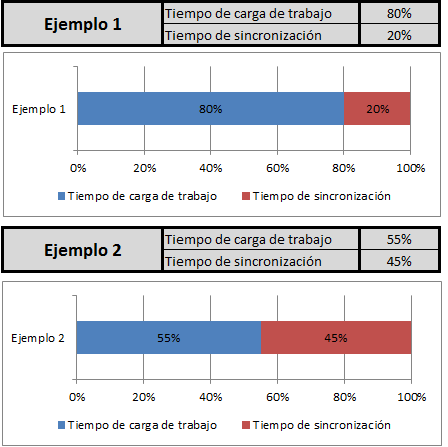
\includegraphics[keepaspectratio]{./resultados_conclusiones/resultados/img/resultados10}
		\caption[Mediciones de escritura de una variable]{Ejemplos de relaciones entre carga de trabajo y tiempo de sincronizaci�n}
		\label{fig:resultados10}
	\end{figure}
	El procesador de Redes de Petri tiene como objetivo reducir el tiempo consumido por la sincronizaci�n y adem�s, facilita la programaci�n de los mecanismos de sincronizaci�n.
	
	En las secciones siguientes se mostrar�n mediciones sobre los tiempos de sincronizaci�n con la utilizaci�n de sem�foros y los tiempos de sincronizaci�n utilizando el procesador de Redes de Petri. Tambi�n, se han realizado mediciones de la carga de trabajo que tiene un sistema Escritor/Escritor, es decir el tiempo consumido en escribir una variable y en cambiar de contexto que todos los hilos trabajen.
	
	\subsection{Medici�n de los tiempos de sincronizaci�n}
		
		En esta secci�n, se muestran las mediciones realizadas sobre los tiempos de sincronizaci�n comparando lo obtenido utilizando sem�foros y utilizando el procesador de Redes de Petri.
		\begin{figure}[H]
			\centering
			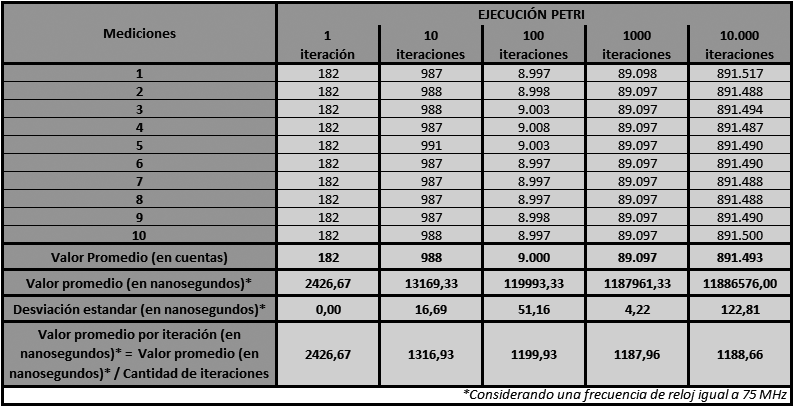
\includegraphics[width=1\linewidth,keepaspectratio]{./resultados_conclusiones/resultados/img/resultados11}
			\caption{Tabla de resultados obtenidos utilizando el procesador de Redes de Petri}
			\label{fig:resultados11}
		\end{figure}
		\begin{figure}[H]
			\centering
			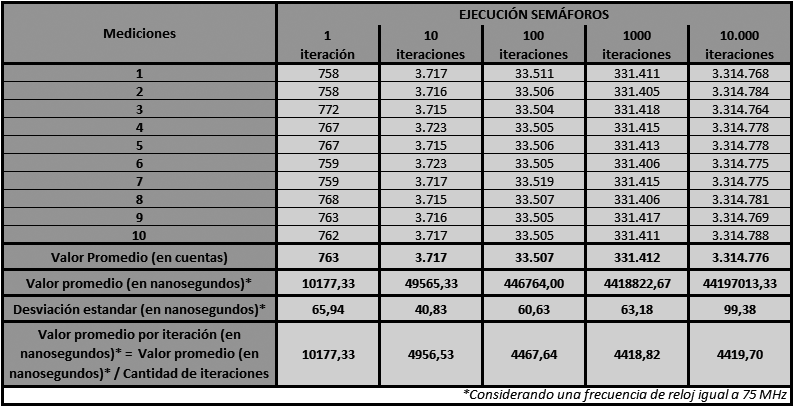
\includegraphics[width=1\linewidth,keepaspectratio]{./resultados_conclusiones/resultados/img/resultados12}
			\caption{Tabla de resultados obtenidos utilizando sem�foros}
			\label{fig:resultados12}
		\end{figure}
		
		Las tablas anteriores (Figuras \ref{fig:resultados11} y \ref{fig:resultados12}), muestran las mediciones realizadas de los tiempos de sincronizaci�n. Para obtener las mediciones de las ejecuciones del procesador de Redes de Petri (Figura \ref{fig:resultados11} se utiliz� el siguiente c�digo.
		
		\begin{lstlisting}
//Iniciar cuenta de tiempo
XTmrCtr_SetControlStatusReg(XPAR_AXI_TIMER_1_BASEADDR,0,0x0);
XTmrCtr_SetLoadReg(XPAR_AXI_TIMER_1_BASEADDR,0,0x00000000);
XTmrCtr_LoadTimerCounterReg(XPAR_AXI_TIMER_1_BASEADDR,0);
ControlStatus=XTmrCtr_GetControlStatusReg(XPAR_AXI_TIMER_1_BASEADDR,0);
XTmrCtr_SetControlStatusReg(XPAR_AXI_TIMER_1_BASEADDR,0,ControlStatus&(~XTC_CSR_LOAD_MASK));
valor_inicial_timer=XTmrCtr_GetTimerCounterReg(XPAR_AXI_TIMER_1_BASEADDR,0);
xil_printf("Valor inicial del timer: %d\r\n\n",valor_inicial_timer);
XTmrCtr_Enable(XPAR_AXI_TIMER_1_BASEADDR, 0);    	

//Procesamiento	
  	for(i=0;i<valor_maximo;i++)
   	{
   		//Pedir T0
   			*(new_disparo_addr) = disparo_t_cero;
   		//Ver si T0 se ejecuto
  			while ( !(*(leer_disparos_ejecutados) & comprobacion_t_cero) )
   			{	}
   		//Sacar T0 de los disparos ejecutados
   			*(sacar_disparo_addr) = disparo_t_cero;
   		//Solicitar el disparo de T1
   			*(new_disparo_addr) = disparo_t_uno;
   		//Ver si T1 se ejecuto
   			while ( !(*(leer_disparos_ejecutados) & comprobacion_t_uno) )
   			{	}
   		//Sacar T1 de los disparos ejecutados
   			*(sacar_disparo_addr) = disparo_t_uno;
   	}
    	
//Terminar cuenta de tiempo
valor_final_timer=XTmrCtr_GetTimerCounterReg(XPAR_AXI_TIMER_1_BASEADDR,0);
xil_printf("Valor final del timer: %d\r\n",valor_final_timer);		
		\end{lstlisting}		
		
		La variable valor m�ximo, como se vi� en la tabla, tom� los valores 1, 10, 100, 1000 y 10000.
			
		En el caso de las mediciones con sem�foros, el c�digo utilizado es el siguiente.
								
		\begin{lstlisting}		
//Iniciar cuenta de tiempo
XTmrCtr_SetControlStatusReg(XPAR_AXI_TIMER_1_BASEADDR,0,0x0);
XTmrCtr_SetLoadReg(XPAR_AXI_TIMER_1_BASEADDR,0,0x00000000);
XTmrCtr_LoadTimerCounterReg(XPAR_AXI_TIMER_1_BASEADDR,0);
ControlStatus=XTmrCtr_GetControlStatusReg(XPAR_AXI_TIMER_1_BASEADDR,0);
XTmrCtr_SetControlStatusReg(XPAR_AXI_TIMER_1_BASEADDR,0,ControlStatus&(~XTC_CSR_LOAD_MASK));
valor_inicial_timer=XTmrCtr_GetTimerCounterReg(XPAR_AXI_TIMER_1_BASEADDR,0);
xil_printf("Valor inicial del timer: %d\r\n\n",valor_inicial_timer);
XTmrCtr_Enable(XPAR_AXI_TIMER_1_BASEADDR, 0); 

//Procesamiento
  	for(i=0;i<valor_maximo;i++)
   	{
   		sem_wait(&semaforo);

   		sem_post(&semaforo);
   	}

//Terminar cuenta de tiempo
valor_final_timer=XTmrCtr_GetTimerCounterReg(XPAR_AXI_TIMER_1_BASEADDR,0);
xil_printf("Valor final timer: %d\r\n",valor_final_timer);	
		\end{lstlisting}
		
		Graficando los datos obtenidos, se observa claramente la reducci�n en los tiempos de sincronizaci�n que produce la utilizaci�n del procesador de redes de Petri.
			  	
		\begin{figure}[H]
			\centering
			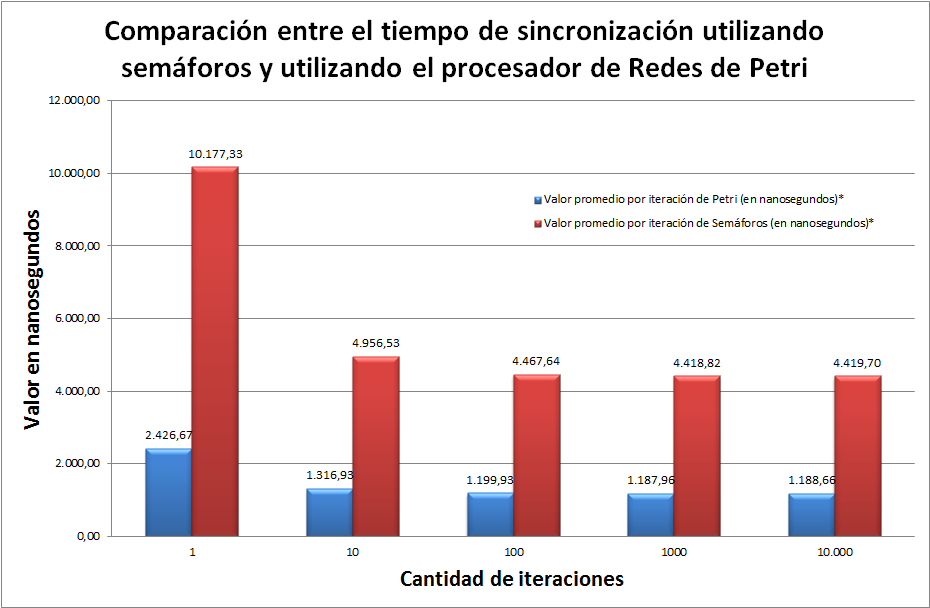
\includegraphics[width=0.85\linewidth,keepaspectratio]{./resultados_conclusiones/resultados/img/resultados13}
			\caption{Comparaci�n del tiempo de sincronizaci�n entre el procesador de Redes de Petri y el uso de Sem�foros}
			\label{fig:resultados13}
		\end{figure}
	
		Mas adelante, luego de haber visto las mediciones de la carga de trabajo, se volver� a apreciar la reducci�n de los tiempos de sincronizaci�n obtenida.
		
	\subsection{Medici�n de la carga de trabajo y duraci�n de cambios de contexto}

		Dada la importancia de la carga de trabajo en las mediciones del rendimiento, estos valores ser�n los primeros que se medir�n.

		Para los problemas que se utilizaron en las mediciones, la carga de trabajo est� determinada por el tiempo de escritura de una variable.
		
		Adem�s, en �stas mediciones, consideramos el peor caso cuando se sincronizan procesos/hilos, �ste caso es, solicitar el disparo de una transici�n y que �sta no pueda ser ejecutada o, hacer una operaci�n \emph{wait} sobre un sem�foro y que el proceso/hilo deba suspenderse. En ambos casos, se producen \emph{cambios de contexto} para que se le asigne tiempo de procesador a un proceso/hilo que s� pueda seguir ejecut�ndose. �sta situaci�n depende del algoritmo del problema que se desea resolver y al sistema sobre el cu�l se lo est� implementando.

		\subsubsection{Escritura de una variable}

			La \textbf{\emph{escritura de la variable}} implica, para este caso, realizar una lectura de la variable, incrementarla y escribir su nuevo valor. �ste procedimiento es utilizado tanto en el problema \emph{escritor/escritor}, (secci�n \ref{sec:problema_escritor}), como en el problema de la \emph{f�brica de mesas} (secci�n \ref{sec:problema_fabrica_mesas}). Por esta raz�n, se realizaron mediciones de la duraci�n de una escritura considerando la repetici�n de 1, 10, 100, 1000 y 10000 escrituras consecutivas. Los valores obtenidos, se muestran en la siguiente tabla.

			\begin{figure}[H]
				\centering
				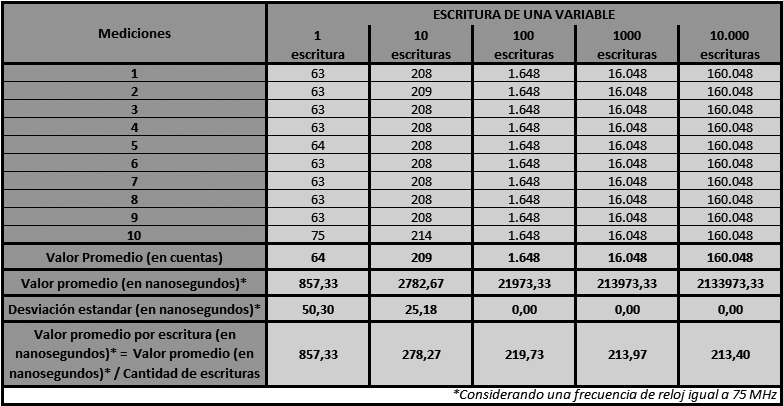
\includegraphics[width=1\linewidth,keepaspectratio]{./resultados_conclusiones/resultados/img/resultados14}
				\caption[Mediciones de escritura de una variable]{Mediciones de escritura de una variable modificando la cantidad de repeticiones de esta acci�n que se realizan en cada ejecuci�n}
				\label{fig:resultados14}
			\end{figure}

			\newpage

			Como se observa en la Figura \ref{fig:resultados14}, en los casos donde se realizaban m�ltiples escrituras consecutivas, se dividi� el tiempo obtenido por la cantidad de escrituras realizadas en ese tiempo. Con estos datos, se obtiene la Figura \ref{fig:resultados15}.
			\begin{figure}[H]
				\centering
				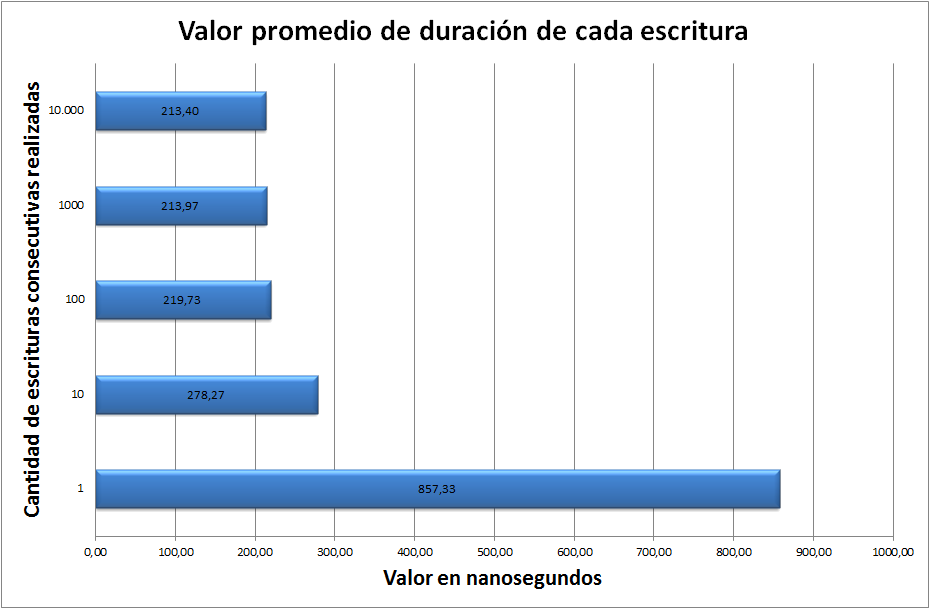
\includegraphics[width=1\linewidth,keepaspectratio]{./resultados_conclusiones/resultados/img/resultados15}
				\caption[Valor promedio de duraci�n de cada escritura]{Valor promedio de duraci�n de cada escritura dependiendo de la cantidad de repeticiones que se realizan en cada ejecuci�n}
				\label{fig:resultados15}
			\end{figure}

			En la Figura \ref{fig:resultados15} se observa que el valor promedio por escritura, se mantiene aproximadamente constante en $0,00021 ms$ a medida que se aumenta la cantidad de cantidad de escrituras consecutivas a realizar por ejecuci�n. La �nica excepci�n se da cuando se mide una �nica escritura.
			
			Para la medici�n de la duraci�n de la escritura de variable, se utiliz� el siguiente c�digo.
			\begin{lstlisting}	
int cuentas = 0;

//Iniciar cuenta de tiempo
XTmrCtr_SetControlStatusReg(XPAR_AXI_TIMER_1_BASEADDR,0,0x0);
XTmrCtr_SetLoadReg(XPAR_AXI_TIMER_1_BASEADDR,0,0x00000000);
XTmrCtr_LoadTimerCounterReg(XPAR_AXI_TIMER_1_BASEADDR,0);
ControlStatus=XTmrCtr_GetControlStatusReg(XPAR_AXI_TIMER_1_BASEADDR,0);
XTmrCtr_SetControlStatusReg(XPAR_AXI_TIMER_1_BASEADDR,0,ControlStatus&(~XTC_CSR_LOAD_MASK));
valor_inicial_timer=XTmrCtr_GetTimerCounterReg(XPAR_AXI_TIMER_1_BASEADDR,0);
xil_printf("Valor inicial del timer: %d\r\n\n",valor_inicial_timer);
XTmrCtr_Enable(XPAR_AXI_TIMER_1_BASEADDR, 0); 

//Escrituras
   	while(cuentas<valor_maximo)
   	{ 	cuentas=cuentas+1; }

//Terminar cuenta de tiempo
valor_final_timer=XTmrCtr_GetTimerCounterReg(XPAR_AXI_TIMER_1_BASEADDR,0);
xil_printf("Valor final del timer: %d\r\n",valor_final_timer);	
			\end{lstlisting}
		 
		\subsubsection{Medici�n de la duraci�n del cambio de contexto}
		
			De manera similar al caso anterior, con dos hilos, se midi� la duraci�n de los \textbf{\emph{cambios de contexto}} entre los hilos. Para ello, se utiliz� la instrucci�n \emph{yield();} que realiza cambio de contexto \cite{xilinx_xilkernel}.
		
			Para la medici�n, se utiliz� el siguiente c�digo.
			\begin{lstlisting}
void* master_thread(void *arg)
{   pthread_attr_t attr;
    pthread_attr_init(&attr);
	pthread_attr_setdetachstate(&attr, PTHREAD_CREATE_JOINABLE);
	int status;
	int *a;
	int *valor_final;

	//Lanzamiendo de los hilos escritores
		status = pthread_create(&hilo_1, &attr, (void*)hilo_medicion_1, NULL);
    	status = pthread_create(&hilo_2, &attr, (void*)hilo_medicion_2, NULL);

    	pthread_join(hilo_1, (void*)&a);
    	pthread_join(hilo_2, (void*)&valor_final);

    xil_printf("Valor final del timer: %d\r\n\n\n", valor_final);
    return (void*)0;
}

/* HILOS */
void* hilo_medicion_1()
{
	int i;
    //Iniciar cuenta de tiempo
	XTmrCtr_SetControlStatusReg(XPAR_AXI_TIMER_1_BASEADDR,0,0x0);
	XTmrCtr_SetLoadReg(XPAR_AXI_TIMER_1_BASEADDR,0,0x00000000);
	XTmrCtr_LoadTimerCounterReg(XPAR_AXI_TIMER_1_BASEADDR,0);
	ControlStatus=XTmrCtr_GetControlStatusReg(XPAR_AXI_TIMER_1_BASEADDR,0);
	XTmrCtr_SetControlStatusReg(XPAR_AXI_TIMER_1_BASEADDR,0,ControlStatus&(~XTC_CSR_LOAD_MASK));
	valor_inicial_timer=XTmrCtr_GetTimerCounterReg(XPAR_AXI_TIMER_1_BASEADDR,0);
	xil_printf("Valor inicial del timer: %d\r\n\n",valor_inicial_timer);
	XTmrCtr_Enable(XPAR_AXI_TIMER_1_BASEADDR, 0); 

	for(i=0;i<cantidad_de_cambios/2;i++)
	{	yield(); }

	pthread_exit((void*)NULL);
	return NULL;
}

void* hilo_medicion_2()
{
	int i;
	for(i=0;i<cantidad_de_cambios/2;i++)
	{	yield(); }
	//Terminar cuenta de tiempo
	valor_final_timer=XTmrCtr_GetTimerCounterReg(XPAR_AXI_TIMER_1_BASEADDR,0);
	pthread_exit((void*)valor_final_timer);
	return NULL;
}
			\end{lstlisting}
		
			Los resultados obtenidos en este caso, fueron:
		
			\begin{figure}[H]
				\centering
				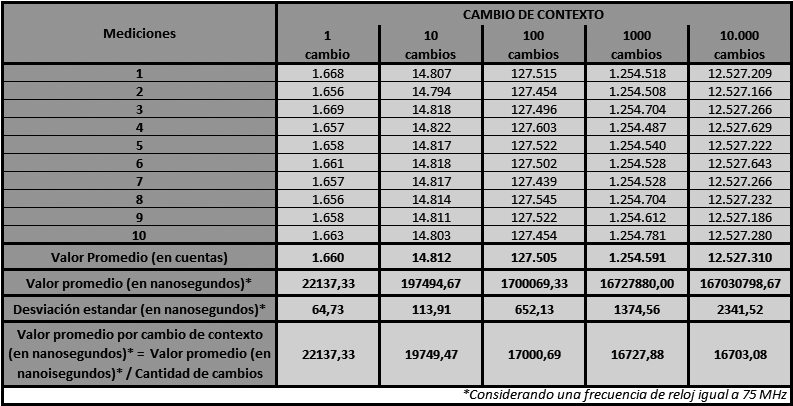
\includegraphics[width=1\linewidth,keepaspectratio]{./resultados_conclusiones/resultados/img/resultados16}
				\caption[Mediciones del cambio de contexto]{Mediciones de duraci�n de los cambios de contexto modificando la cantidad de repeticiones de esta acci�n que se realizan en cada ejecuci�n}
				\label{fig:resultados16}
			\end{figure}
			
			\newpage
			
			\begin{figure}[H]
				\centering
				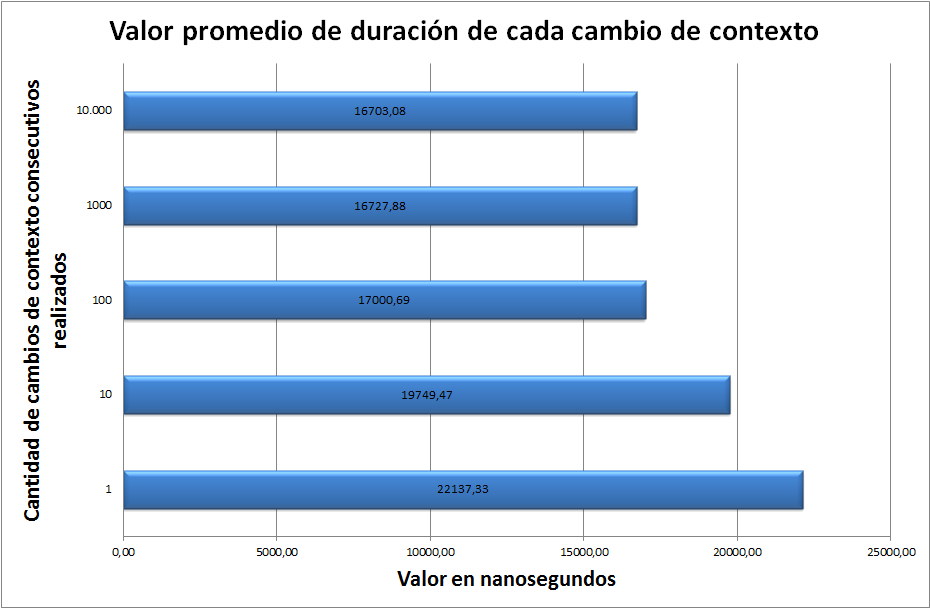
\includegraphics[width=1\linewidth,keepaspectratio]{./resultados_conclusiones/resultados/img/resultados17}
				\caption[Valor promedio de duraci�n de cada cambio de contexto]{Valor promedio de duraci�n de cada cambio de contexto dependiendo de la cantidad de repeticiones que se realizan en cada ejecuci�n}
				\label{fig:resultados17}
			\end{figure}
			
		\subsubsection{An�lisis de los resultados obtenidos}
		
			En resumen, con los valores medidos de carga de trabajo y de tiempos de sincronizaci�n, es posible armar un gr�fico similar a los de la Figura \ref{fig:resultados10}.
		
			De �sta manera, es posible apreciar la reducci�n en tiempo de sincronizaci�n que entrega el procesador de Redes de Petri con respecto a la carga de trabajo del sistema (figuras \ref{fig:resultados18} y \ref{fig:resultados19}).
			
			Como se observa en las figuras \ref{fig:resultados18} y \ref{fig:resultados19}, el uso de sem�foros, hace que el tiempo de sincronizaci�n sea aproximadamente el $20\%$ de tiempo total. Por otro lado, se verifica que el uso del procesador de Redes de Petri logra reducir �ste tiempo de sincronizaci�n hasta aproximadamente un $10\%'$ del tiempo total.
			
			\newpage
			
			\begin{figure}[H]
				\centering
				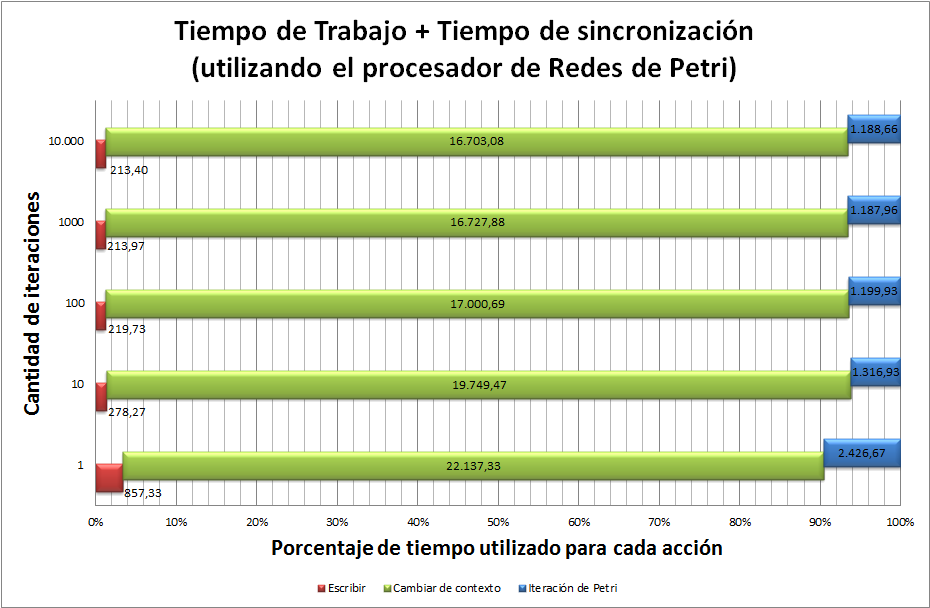
\includegraphics[width=0.85\linewidth,keepaspectratio]{./resultados_conclusiones/resultados/img/resultados18}
				\caption{Carga de trabajo m�s sincronizaci�n utilizando el procesador de Redes de Petri}
				\label{fig:resultados18}
			\end{figure}
			\begin{figure}[H]
				\centering
				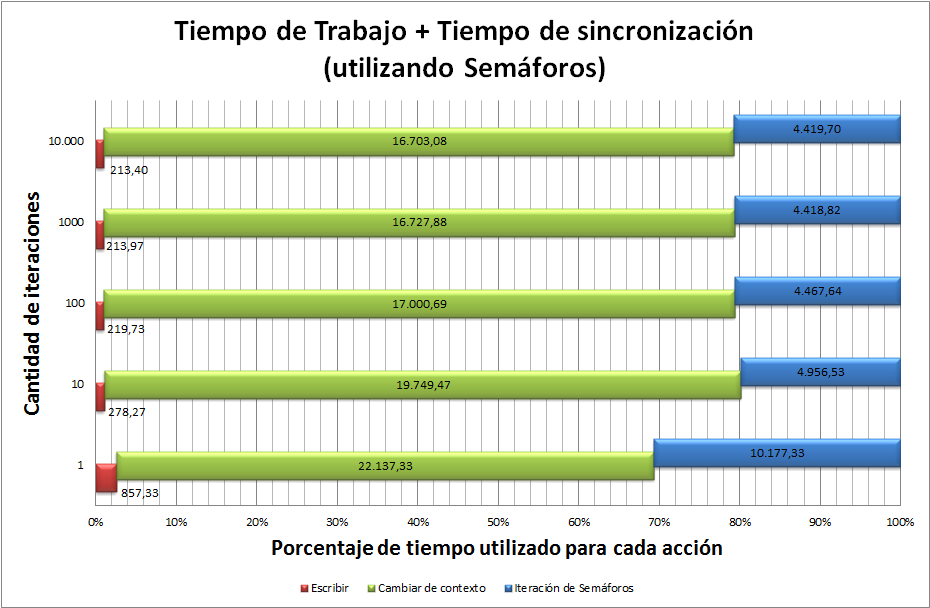
\includegraphics[width=0.85\linewidth,keepaspectratio]{./resultados_conclusiones/resultados/img/resultados19}
				\caption{Carga de trabajo m�s sincronizaci�n utilizando Sem�foros}
				\label{fig:resultados19}
			\end{figure}
			
			\begin{quote}
				\textbf{\emph
				{
					En resumen, el procesador de Redes de Petri cumple su objetivo de reducir el porcentaje de tiempo que se consume 
					para controlar la sincronizaci�n dentro de un sistema.
				}}
			\end{quote}
				
	
	% Interrupciones en el procesador de Redes de Petri
		%%%%%%%%%%%%%%%%%%%%%%%%%%%%%%%%%%%%%%%%%%%%%%%%%%%%%%%%%%%%%%%%%%%%%%%%%%%%%%%%%%%%%
%																					%
%	TRABAJO: Proyecto Integrador													%
%																					%
%		Titulo: 	Desarrollo de IP cores con procesamiento de Redes de Petri 		%
%					Temporales para sistemas multicore en FPGA						%
%																					%
%		Autores:	Juli�n Nonino													%
%					Carlos Renzo Pisetta											%
%		Director:	Orlando Micolini												%
%																					%
%	Parte: Resultados y Conclusiones												%
%	Capitulo: Resultados															%
%	Seccion: Interrupciones en el procesador de Redes de Petri						%	
%	Archivo: resultados_interrupciones.tex											%
%																					%
%%%%%%%%%%%%%%%%%%%%%%%%%%%%%%%%%%%%%%%%%%%%%%%%%%%%%%%%%%%%%%%%%%%%%%%%%%%%%%%%%%%%%

% Path Imagenes: ./resultado_conclusiones/resultados/img
% Nombre predeterminado imagenes: resultadosxx
%	xx es el numero de imagen	

\section{Interrupciones en el procesador de Redes de Petri}
	\label{sec:resultados_interrupciones}
	
	El procesador de Redes de Petri, es capaz de generar interrupciones notificando a los hilos/procesos que
	un disparo ha sido ejecutado, por �sta raz�n, en �sta secci�n, presentamos mediciones sobre como afecta
	al rendimiento del sistema el uso de interrupciones en lugar de los otros m�todos de espera.
			
	Para las mediciones, se utiliz� la siguiente Red de Petri (Figura \ref{fig:resultados20}). En dicha Figura, 
	se muestra la red con las diferentes cantidades de tokens en la plaza $P0$. 
			
	\begin{figure}[H]
		\centering
		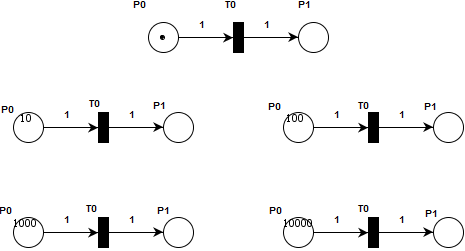
\includegraphics[width=1\linewidth,keepaspectratio]{./resultados_conclusiones/resultados/img/resultados20}
		\caption{Red de Petri utilizada para la medici�n de las interrupciones}
		\label{fig:resultados20}
	\end{figure}
	
	\newpage		
			
	Luego, se se arm� la siguiente tabla con los valores obtenidos.
	
	\begin{figure}[H]
		\centering
		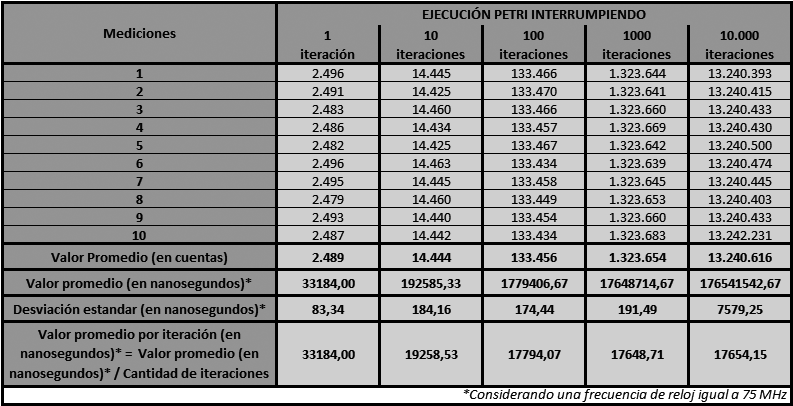
\includegraphics[width=0.9\linewidth,keepaspectratio]{./resultados_conclusiones/resultados/img/resultados21}
		\caption{Tabla de resultados obtenidos utilizando el procesador de Redes de Petri con interrupciones}
		\label{fig:resultados21}
	\end{figure}
	\begin{figure}[H]
		\centering
		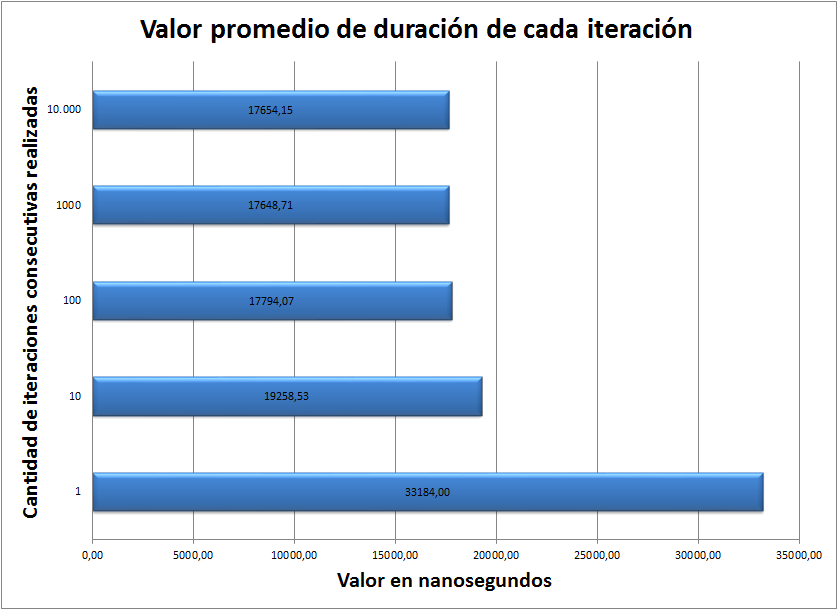
\includegraphics[width=0.9\linewidth,keepaspectratio]{./resultados_conclusiones/resultados/img/resultados22}
		\caption{Valor promedio de duraci�n de cada iteraci�n dependiendo de la cantidad de repeticiones que se realizan en cada ejecuci�n}
		\label{fig:resultados22}
	\end{figure}			
	
	A continuaci�n, se repetir�n las gr�ficas de las Figuras \ref{fig:resultados18} y \ref{fig:resultados19} pero, comparando
	el procesador de Redes de Petri CON y SIN interrupciones.
	
	\begin{figure}[H]
		\centering
		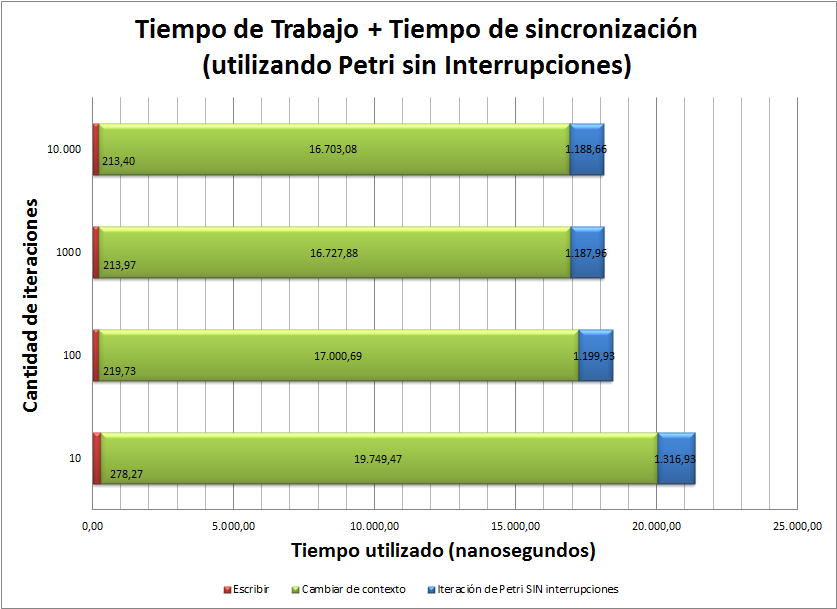
\includegraphics[width=0.8\linewidth,keepaspectratio]{./resultados_conclusiones/resultados/img/resultados23}
		\caption{Carga de trabajo m�s sincronizaci�n utilizando el procesador de Redes de Petri SIN interrupciones}
		\label{fig:resultados23}
	\end{figure}
	\begin{figure}[H]
		\centering
		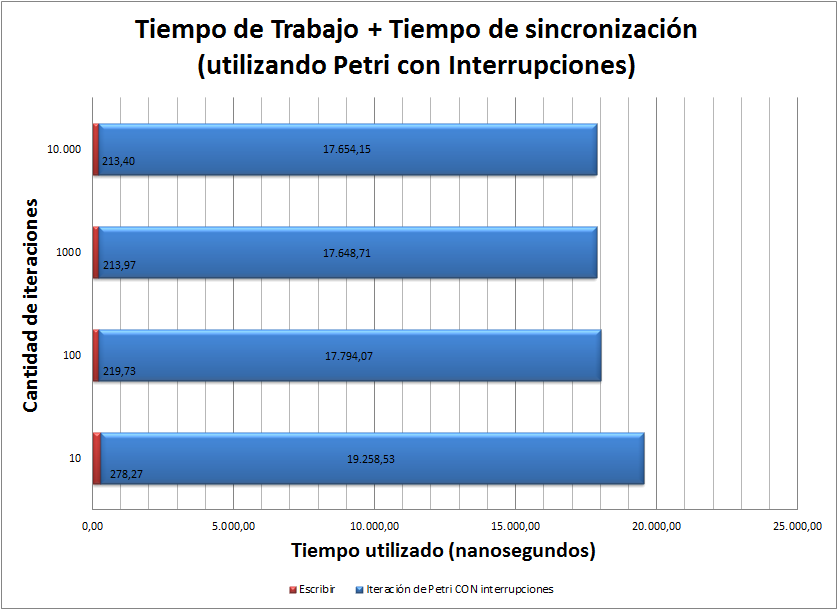
\includegraphics[width=0.8\linewidth,keepaspectratio]{./resultados_conclusiones/resultados/img/resultados24}
		\caption{Carga de trabajo m�s sincronizaci�n utilizando el procesador de Redes de Petri CON interrupciones}
		\label{fig:resultados24}
	\end{figure}
	
	Se debe notar que en la gr�fica con los datos de las interrupciones (Figura \ref{fig:resultados24}) no se incluye
	la duraci�n de un cambio de contexto. �sto se debe a que al utilizar interrupciones, el proceso se suspende siempre
	y se produce un cambio de contexto al llegar la interrupci�n y otro al darle el control nuevamente al hilo, ya reactivado,
	para que siga su funci�n. Por ello, la duraci�n del cambio de contexto est� incluida dentro del tiempo de sincronizaci�n
	consumido por el procesador de Redes de Petri.
	
	En las Figuras \ref{fig:resultados23} y \ref{fig:resultados24} se observa que el uso de interrupciones hace que
	la carga de trabajo de escribir una variable m�s el tiempo de sincronziaci�n sea aproximadamente $1000$ nanosegundos
	menor que sin utilizar interrupciones.
		
		
	% Problema escritores
		%%%%%%%%%%%%%%%%%%%%%%%%%%%%%%%%%%%%%%%%%%%%%%%%%%%%%%%%%%%%%%%%%%%%%%%%%%%%%%%%%%%%%
%																					%
%	TRABAJO: Proyecto Integrador													%
%																					%
%		Titulo: 	Desarrollo de IP cores con procesamiento de Redes de Petri 		%
%					Temporales para sistemas multicore en FPGA						%
%																					%
%		Autores:	Juli�n Nonino													%
%					Carlos Renzo Pisetta											%
%		Director:	Orlando Micolini												%
%																					%
%	Parte: Resultados y Conclusiones												%
%	Capitulo: Resultados															%
%	Seccion: Problema: Escritor/Escritor											%	
%	Archivo: problema_escritor.tex													%
%																					%
%%%%%%%%%%%%%%%%%%%%%%%%%%%%%%%%%%%%%%%%%%%%%%%%%%%%%%%%%%%%%%%%%%%%%%%%%%%%%%%%%%%%%

% Path Imagenes: ./resultado_conclusiones/resultados/img
% Nombre predeterminado imagenes: resultadosxx
%	xx es el numero de imagen

\section{Problema: \emph{Escritor/Escritor}}
	\label{sec:problema_escritor}

	Para realizar estas mediciones se utiliz� un sistema con una variable compartida por varios hilos que
	desean escribirla. �sta situaci�n se conoce como problema del Escritor/Escritor.

	\subsection{Modelo del problema}

		En �sta secci�n se presentar� el modelo del problema Escritor/Escritor con una Red de Petri.
		Como se realizar�n pruebas con 2, 3, 4 y 5 hilos se realizar�n cuatro Redes de Petri.
		\begin{figure}[H]
			\centering
			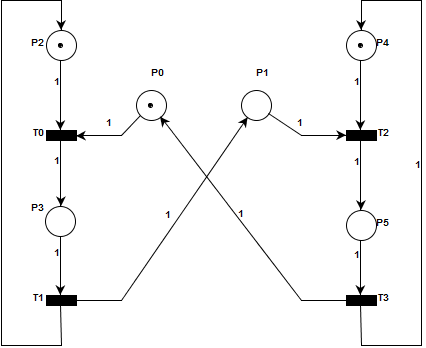
\includegraphics[width=0.7\linewidth,keepaspectratio]{./resultados_conclusiones/resultados/img/resultados25}
			\caption{Red de Petri Escritor/Escritor (2 hilos)}
			\label{fig:resultados25}
		\end{figure}
		
		\newpage
		
		\begin{figure}[H]
			\centering
			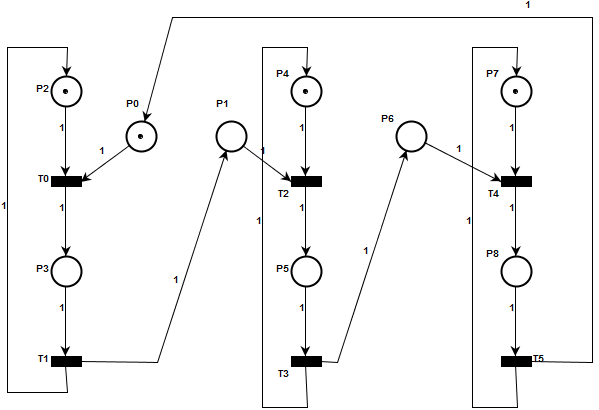
\includegraphics[width=1\linewidth,keepaspectratio]{./resultados_conclusiones/resultados/img/resultados26}
			\caption{Red de Petri Escritor/Escritor (3 hilos)}
			\label{fig:resultados26}
		\end{figure}

		\begin{figure}[H]
			\centering
			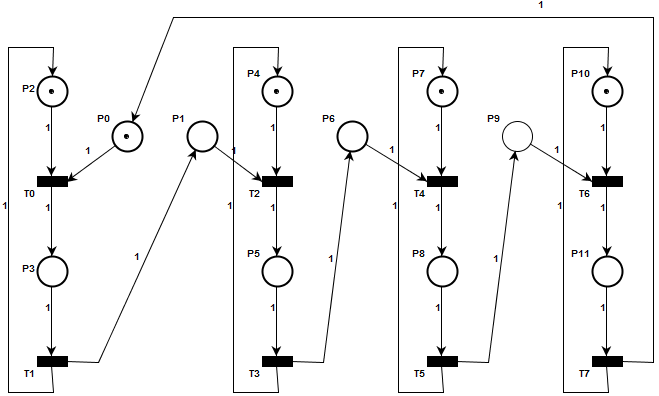
\includegraphics[width=1\linewidth,keepaspectratio]{./resultados_conclusiones/resultados/img/resultados27}
			\caption{Red de Petri Escritor/Escritor (4 hilos)}
			\label{fig:resultados27}
		\end{figure}
		
		\newpage
		
		\begin{figure}[H]
			\centering
			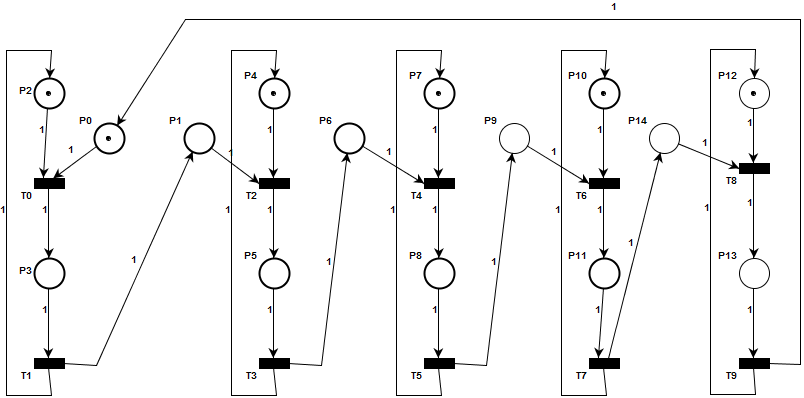
\includegraphics[width=1\linewidth,keepaspectratio]{./resultados_conclusiones/resultados/img/resultados28}
			\caption{Red de Petri Escritor/Escritor (5 hilos)}
			\label{fig:resultados28}
		\end{figure}

	\subsection{Secuencia de ejecuci�n utilizando sem�foros}

		La secuencia de ejecuci�n del programa en C dise�ado para resolver este problema utilizando
		sem�foros es la siguiente:
		\begin{enumerate}
		  	\item Creaci�n del sem�foro.
		  	\item Creaci�n de los hilos. Se realizar�n cuatro implementaciones con 2, 3, 4 y 5 hilos en
		  		ejecuci�n.
		  	\item Cada hilo intenta solicitar el permiso por parte del sem�foro. Al conseguirlo, incrementa
		  		la variable compartida. Luego, libera el sem�foro. Esta operaci�n se repetir� 10, 100, 1000 y
		  		10000 veces en diferentes ejecuciones.
		  	\item Una vez que se ha realizado la cantidad de iteraciones especificada, se detienen los hilos.
		  	\item Se detiene el timer.
		\end{enumerate}
		El c�digo fuente del programa puede ser encontrado en el ap�ndice \ref{ap:codigos_programas}, en la secci�n
		\ref{sec:programa_escritor_sem}, p�gina \pageref{sec:programa_escritor_sem}.
	
	\subsection{Secuencia de ejecuci�n utilizando el procesador de Redes de Petri}

		La secuencia de ejecuci�n del programa en \emph{C} dise�ado para resolver este problema
		utilizando el procesador de Redes de Petri como motor de sincronizaci�n es la siguiente:
		\begin{enumerate}
		  	\item Carga del marcado inicial.
		  	\item Carga de la matriz de incidencia.
		  	\item Carga de la matriz de inhibici�n.
		  	\item Carga del vector de cotas de plazas.
		  	\item Carga del vector de transiciones autom�ticas.
		  	\item Carga del vector EFT (Earliest Firing Time).
		  	\item Carga del vector de incrementos de tiempo.
		  	\item Carga del vector LFT (Latest Firing Time).
		  	\item Creaci�n de los hilos. Se realizar�n cuatro implementaciones con 2, 3, 4 y 5 hilos en
		  		ejecuci�n.
		  	\item Cada hilo intenta solicitar el permiso para escribir la variable solicitando al procesador
		  		de Petri el disparo de la transici�n para pedir la exclusi�n mutua. Luego, el proceso espera
		  		verificando hasta que su solicitud haya sido ejecutada. Cuando el disparo se ejecuto,
		  		incrementa la variable compartida. Luego, solicita el disparo de una segunda transici�n para
		  		devolver el token de exclusi�n mutua. Esta operaci�n se repetir� 10, 100, 1000 y
		  		10000 veces en diferentes ejecuciones.
		  	\item Una vez que se ha realizado la cantidad de iteraciones especificada, se detienen los hilos.
		  	\item Se detiene el timer.
		\end{enumerate}
		El c�digo fuente del programa puede ser encontrado en el ap�ndice \ref{ap:codigos_programas}, en la secci�n
		\ref{sec:programa_escritor_petri}, p�gina \pageref{sec:programa_escritor_petri}.

	\newpage
			
	\subsection{Mediciones realizadas}
		
		\subsubsection{Mediciones realizadas con dos (2) hilos escritores}
								
			Para un sistema con dos hilos corriendo, se tomaron mediciones de 10, 100, 1000 y 10000
			iteraciones. Los datos obtenidos son (Figura \ref{fig:resultados29}):
			\begin{figure}[H]
				\centering
				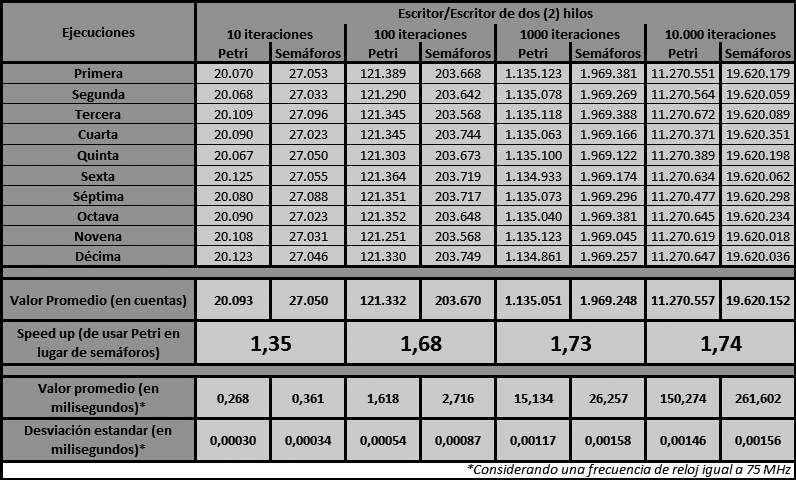
\includegraphics[width=0.8\linewidth,keepaspectratio]{./resultados_conclusiones/resultados/img/resultados29}
				\caption{Tabla de mediciones realizadas para dos hilos en ejecuci�n}
				\label{fig:resultados29}
			\end{figure}

		\subsubsection{Mediciones realizadas con tres (3) hilos escritores}
							
			Para un sistema con tres hilos corriendo, se tomaron mediciones de 10, 100, 1000 y 10000
			iteraciones.
			Los datos obtenidos son (Figura \ref{fig:resultados30}):
			\begin{figure}[H]
				\centering
				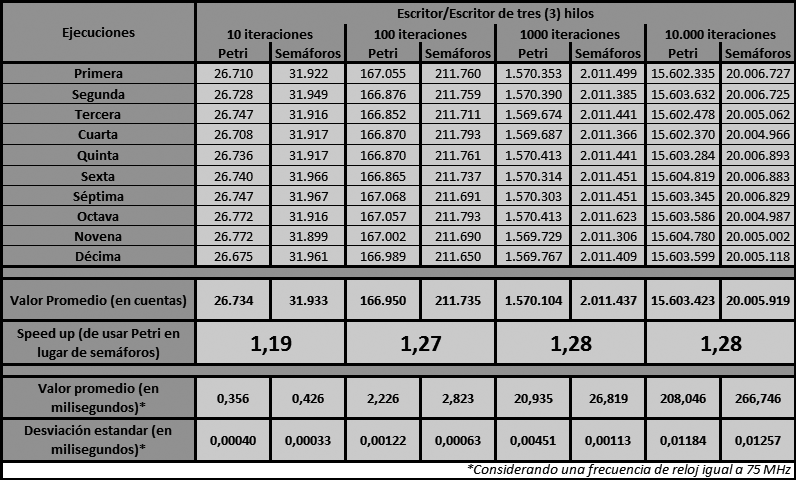
\includegraphics[width=0.8\linewidth,keepaspectratio]{./resultados_conclusiones/resultados/img/resultados30}
				\caption{Tabla de mediciones realizadas para tres hilos en ejecuci�n}
				\label{fig:resultados30}
			\end{figure}
		
		\subsubsection{Mediciones realizadas con cuatro (4) hilos escritores}
							
			Para un sistema con cuatro hilos corriendo, se tomaron mediciones de 10, 100, 1000 y 10000
			iteraciones.
			Los datos obtenidos son (Figura \ref{fig:resultados31}):
			\begin{figure}[H]
				\centering
				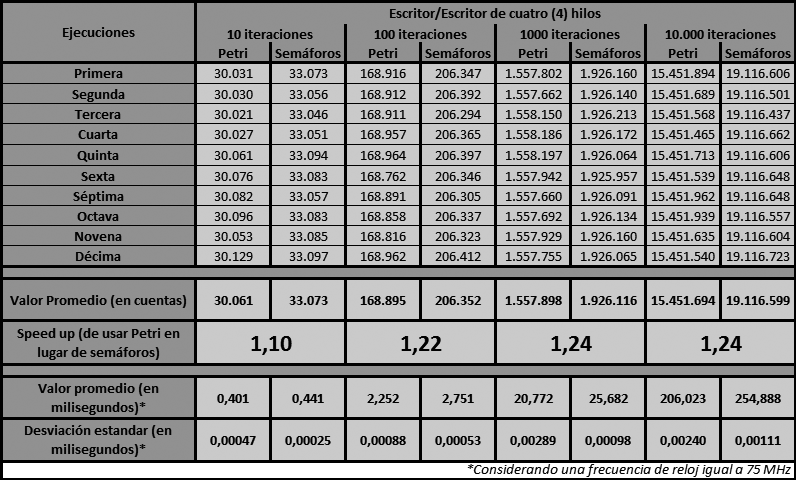
\includegraphics[width=0.8\linewidth,keepaspectratio]{./resultados_conclusiones/resultados/img/resultados31}
				\caption{Tabla de mediciones realizadas para cuatro hilos en ejecuci�n}
				\label{fig:resultados31}
			\end{figure}

		\subsubsection{Mediciones realizadas con cinco (5) hilos escritores}
			
			Para un sistema con cinco hilos corriendo, se tomaron mediciones de 10, 100, 1000 y 10000
			iteraciones.
			Los datos obtenidos son (Figura \ref{fig:resultados32}):
			\begin{figure}[H]
				\centering
				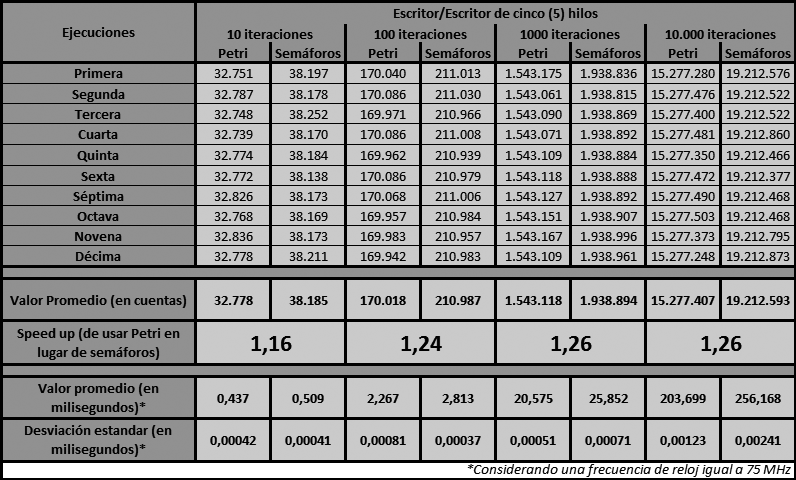
\includegraphics[width=0.8\linewidth,keepaspectratio]{./resultados_conclusiones/resultados/img/resultados32}
				\caption{Tabla de mediciones realizadas para cinco hilos en ejecuci�n}
				\label{fig:resultados32}
			\end{figure}
		
	\subsection{An�lisis de los resultados obtenidos}
		
		Con los datos mostrados en la secci�n anterior, se arm� una gr�fica que muestra el incremento en velocidad
		(\emph{speed up}) que se consigue al utilizar el procesador de Redes de Petri en lugar de sem�foros para
		sincronizar procesos.
		
		\begin{figure}[H]
			\centering
			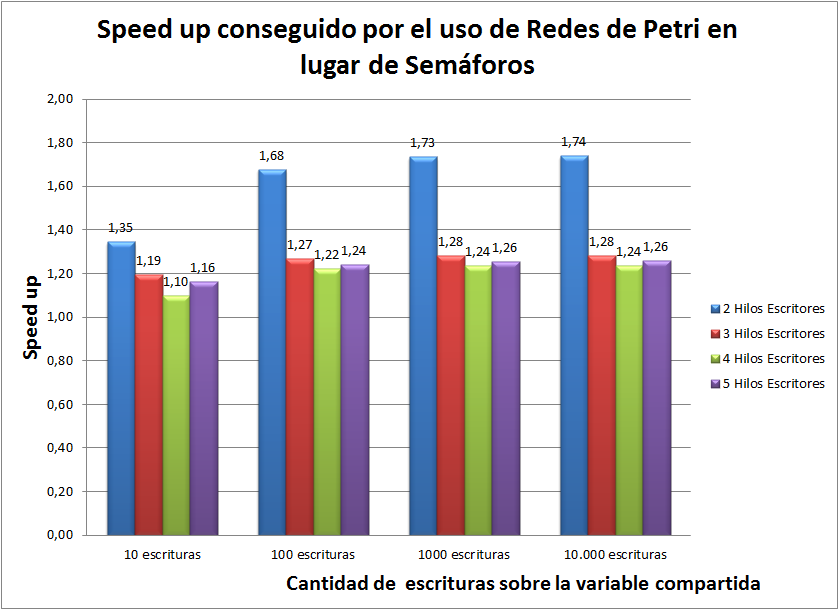
\includegraphics[width=0.85\linewidth,keepaspectratio]{./resultados_conclusiones/resultados/img/resultados33}
			\caption{Speed up de utilizar el procesador de Redes de Petri frente al uso de Sem�foros}
			\label{fig:resultados33}
		\end{figure}
		
		Las tablas mostradas anteriormente y la Figura \ref{fig:resultados33} que resume los datos, muestran que el
		\textbf{\emph{procesador de Redes de Petri en promedio es entre un $\boldsymbol{15\%}$ y un $\boldsymbol{30\%}$ 
		m�s r�pido que el uso de sem�foros}} para resolver el problema de sincronizar m�ltiples hilos que desean escribir 
		sobre una variable compartida. Incluso, se \textbf{\emph{alcanzan picos de hasta un $\boldsymbol{70\%}$ de mayor 
		velocidad}}.
	
	\subsection{Comparaci�n entre las diferentes maneras de esperar la ejecuci�n de los disparos}
	
		Como se dijo en la secci�n \ref{sec:programacion}, existen tres formas de que un proceso/hilo espere  que el disparo
		que solicit� sea ejecutado. �stos son:
		\begin{itemize}
		  	\item Esperar activamente.
		  	\item Ceder el procesador si el disparo a�n no esta listo.
		  	\item Suspenderse y que cuando el procesador de Redes de Petri resuelva el disparo genere una interrupci�n
		  		lo reactive.
		\end{itemize}
		
		\newpage
		
		En dicha secci�n, tambi�n se dijo que para el problema Escritor/Escritor, no era conveniente que se realizara una
		espera activa porque ello llevar�a a un desaprovechamiento del tiempo del procesador. �sto se debe a que como los
		escritores escriben secuencialmente, luego de que uno de ellos lo haga, no podr� volver a hacerlo hasta que el resto
		de los escritores escriba.
		
		En la Figura \ref{fig:resultados34} se observa la situaci�n mencionada anteriormente. Utilizar la funci�n \emph{yield()}
		o, un sistema de interrupciones es por lo menos $400$ veces mejor que esperar activamente consumiendo tiempo del procesador.
		
		En cuanto a la comparaci�n entre la utilizaci�n del \emph{yield()} y el uso de interrupciones, el primero, mantiene al
		hilo en la planificaci�n del sistema operativo, por lo tanto, si se le otorga tiempo del procesador nuevamente y su
		disparo a�n no ha sido ejecutado volver� a ceder el paso, provocando un nuevo cambio de contexto. Por �sta raz�n, en 
		casos donde, por ejemplo las transiciones NO tienen restricciones temporales para ser ejecutados, el uso de 
		interrupciones tiene un peor desempe�o que el uso de la funci�n \emph{yield()} como sucede en �ste problema.
		
		\begin{figure}[H]
			\centering
			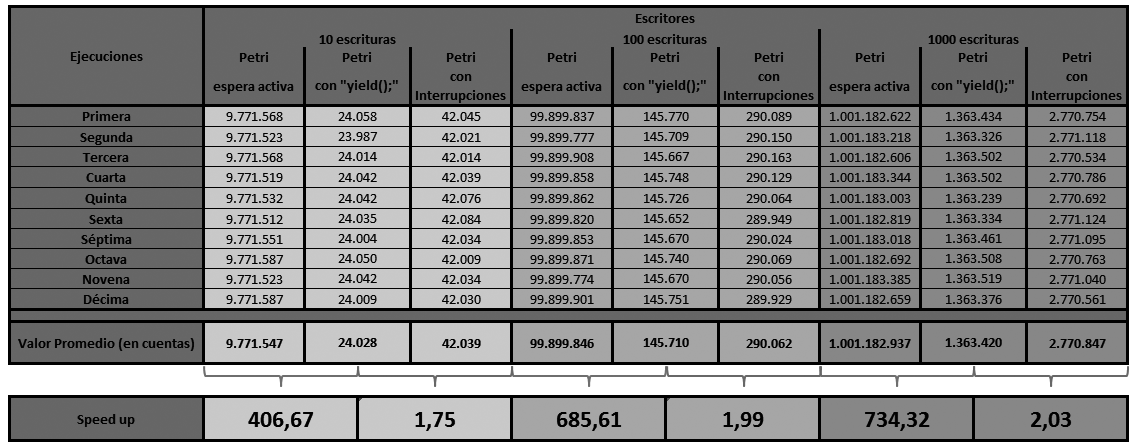
\includegraphics[width=1\linewidth,keepaspectratio]{./resultados_conclusiones/resultados/img/resultados34}
			\caption{Tabla comparativa de los distintos m�todos de espera de disparos para el problema Escritor/Escritor}
			\label{fig:resultados34}
		\end{figure}
			
		
		
	% Problema fabrica de mesas
		%%%%%%%%%%%%%%%%%%%%%%%%%%%%%%%%%%%%%%%%%%%%%%%%%%%%%%%%%%%%%%%%%%%%%%%%%%%%%%%%%%%%%
%																					%
%	TRABAJO: Proyecto Integrador													%
%																					%
%		Titulo: 	Desarrollo de IP cores con procesamiento de Redes de Petri 		%
%					Temporales para sistemas multicore en FPGA						%
%																					%
%		Autores:	Juli�n Nonino													%
%					Carlos Renzo Pisetta											%
%		Director:	Orlando Micolini												%
%																					%
%	Parte: Resultados y Conclusiones												%
%	Capitulo: Resultados															%
%	Seccion: Problema: F�brica de Mesas												%	
%	Archivo: problema_fabrica_mesas.tex												%
%																					%
%%%%%%%%%%%%%%%%%%%%%%%%%%%%%%%%%%%%%%%%%%%%%%%%%%%%%%%%%%%%%%%%%%%%%%%%%%%%%%%%%%%%%

% Path Imagenes: ./resultado_conclusiones/resultados/img
% Nombre predeterminado imagenes: resultadosxx
%	xx es el numero de imagen

\section{Problema: \emph{F�brica de Mesas}}
	\label{sec:problema_fabrica_mesas}
		
	El problema de la f�brica de mesas, ha sido inventado para �ste trabajo con el objetivo de verificar el funcionamiento
	del procesador de Redes de Petri Temporizadas, como se vi� en la secci�n \ref{sec:fabrica_mesas}, p�gina \pageref{sec:fabrica_mesas}.
	
	La idea fundamentalmente es crear una l�nea de producci�n donde en cada etapa existan repositorios de recursos (\emph{variables})
	y trabajadores (\emph{hilos/procesos}) accedan a ellos, realicen un procesamiento  sobre los mismos con una determinada
	duraci�n.
	
	\newpage
		
	\subsection{Modelo del problema}
			
		Modelando el problema, se obtiene la siguiente Red de Petri (Figura \ref{fig:resultados35}).
		\begin{figure}[H]
			\centering
			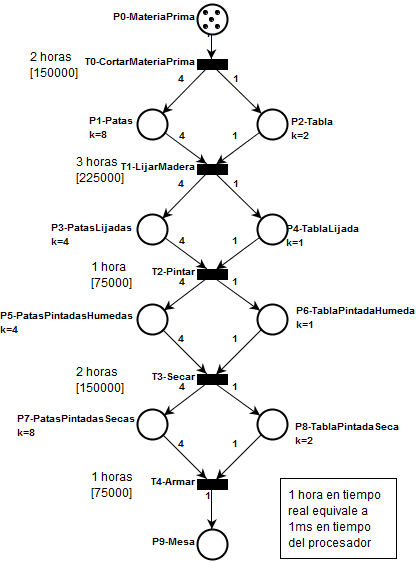
\includegraphics[width=0.9\linewidth,keepaspectratio]{./resultados_conclusiones/resultados/img/resultados35}
			\caption{Red de Petri que modela el problema de la f�brica de mesas}
			\label{fig:resultados35}
		\end{figure}
	
	\newpage
			
	\subsection{Mediciones realizadas}
		
		Utilizando los c�digos fuentes incluidos en el ap�ndice \ref{ap:codigos_programas}, para la ejecuci�n con
		sem�foros el mostrado en la secci�n \ref{sec:programa_fabrica_mesas_sem} de la p�gina \pageref{sec:programa_fabrica_mesas_sem},
		y, para la ejecuci�n con Redes de Petri el c�digo de la secci�n \ref{sec:programa_fabrica_mesas_petri} de la
		p�gina \pageref{sec:programa_fabrica_mesas_petri}.
		
		\begin{figure}[H]
			\centering
			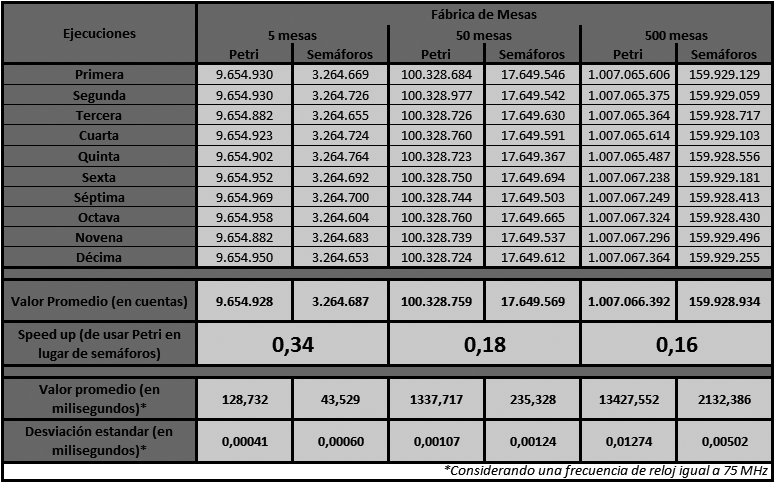
\includegraphics[width=1\linewidth,keepaspectratio]{./resultados_conclusiones/resultados/img/resultados36}
			\caption{Tabla de mediciones realizadas para el problema de la f�brica de mesas}
			\label{fig:resultados36}
		\end{figure}
			
	\subsection{An�lisis de los resultados obtenidos}
	
		La imagen anterior, muestra que el procesador de Redes de Petri tiene un peor desempe�o que la resoluci�n con
		sem�foros. �sto, se debe a que la resoluci�n con Redes de Petri utiliza interrupciones, lo que implica que se 
		debe suspender al hilo mientras espera que su disparo sea realizado. El problema es que, con el sistema operativo
		utilizado (Xilkernel), la �nica manera de suspender un hilo y quitarlo de la planificaci�n de procesos es utilizar
		sem�foros. Por �sta raz�n, no es posible hacer una comparaci�n adecuada entre el procesador de Redes de Petri y la 
		resoluci�n utilizando sem�foros debido a que el programa que utiliza el procesador de Redes de Petri tambi�n debe
		utilizar sem�foros.
		
		Adem�s, cada interrupci�n que se produce implica que se cambie de contexto hacia el proceso encargado de atender
		la interrupci�n y luego, se vuelva a darle el control a los hilos del sistema. �sto tambi�n genera que el valor
		de tiempo medido al resolver el problema con el procesador de Redes de Petri aumente.
					
		
	% Problema fabrica de mesas
		%%%%%%%%%%%%%%%%%%%%%%%%%%%%%%%%%%%%%%%%%%%%%%%%%%%%%%%%%%%%%%%%%%%%%%%%%%%%%%%%%%%%%
%																					%
%	TRABAJO: Proyecto Integrador													%
%																					%
%		Titulo: 	Desarrollo de IP cores con procesamiento de Redes de Petri 		%
%					Temporales para sistemas multicore en FPGA						%
%																					%
%		Autores:	Juli�n Nonino													%
%					Carlos Renzo Pisetta											%
%		Director:	Orlando Micolini												%
%																					%
%	Parte: Resultados y Conclusiones												%
%	Capitulo: Resultados															%
%	Seccion: Problema: Cena de los Fil�sofos										%	
%	Archivo: problema_cena_filosofos.tex											%
%																					%
%%%%%%%%%%%%%%%%%%%%%%%%%%%%%%%%%%%%%%%%%%%%%%%%%%%%%%%%%%%%%%%%%%%%%%%%%%%%%%%%%%%%%

% Path Imagenes: ./resultado_conclusiones/resultados/img
% Nombre predeterminado imagenes: resultadosxx
%	xx es el numero de imagen	
		
\section{Problema: \emph{Cena de los Fil�sofos}}
	\label{sec:problema_cena_filosofos}
		
	El problema de los fil�sofos cenando es un problema cl�sico de las ciencias de la computaci�n propuesto por \emph{Edsger 
	Dijkstra} en 1965 para representar el problema de la sincronizaci�n de procesos en un sistema operativo. Cabe aclarar 
	que la interpretaci�n est� basada en pensadores chinos, quienes com�an con dos palillos, donde es m�s l�gico que se 
	necesite el del comensal que se siente al lado para poder comer\footnotemark[\value{footnote}].
	
	\subsection{Enunciado del problema}
		
		Cinco fil�sofos se sientan alrededor de una mesa y pasan su vida cenando y pensando. Cada fil�sofo tiene un plato de 
		comida y un tenedor a la izquierda de su plato. Para comer son necesarios dos tenedores y cada fil�sofo s�lo puede 
		tomar los que est�n a su izquierda y derecha. Si cualquier fil�sofo coge un tenedor y el otro est� ocupado, se quedar� 
		esperando, con el tenedor en la mano, hasta que pueda coger el otro tenedor, para luego empezar a comer.
		
		Si dos fil�sofos adyacentes intentan tomar el mismo tenedor a una vez, se produce una condici�n de carrera: ambos 
		compiten por tomar el mismo tenedor, y uno de ellos se queda sin comer.
		
		Si todos los fil�sofos toman el tenedor que est� a su derecha al mismo tiempo, entonces todos se quedar�n esperando 
		eternamente, porque alguien debe liberar el tenedor que les falta. Nadie lo har� porque todos se encuentran en la 
		misma situaci�n (esperando que alguno deje sus tenedores). Entonces los fil�sofos se morir�n de hambre. Este bloqueo 
		mutuo se denomina interbloqueo o deadlock.
		
		El problema consiste en encontrar un algoritmo que permita que los fil�sofos nunca se mueran de hambre\footnotemark[\value{footnote}].
		
		\footnotetext[\value{footnote}]{Texto extra�do del sitio web \url{http://es.wikipedia.org/wiki/Problema_de_la_cena_de_los_filosofos}}
			
	\subsection{Modelo del problema}
	
		Modelando el problema, se obtiene la Red de Petri de la Figura \ref{fig:resultados37}. Para �ste caso, s�lo se
		utilizar�n tres ($3$) fil�sofos.
		
		\newpage
		
		\begin{figure}[H]
			\centering
			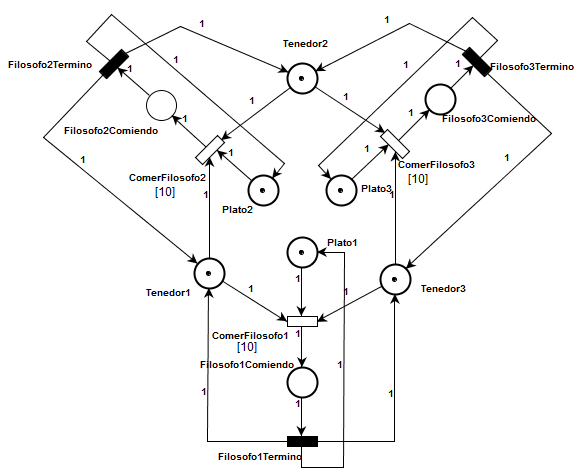
\includegraphics[width=0.75\linewidth,keepaspectratio]{./resultados_conclusiones/resultados/img/resultados37}
			\caption{Red de Petri que modela el problema de la cena de los fil�sofos}
			\label{fig:resultados37}
		\end{figure}

	\subsection{Mediciones realizadas y an�lisis de resultados}
	
		Como ya se ha determinado que si se utilizan interrupciones no hay comparaci�n con la resoluci�n que
		utiliza sem�foros, para �ste problema se decidi� medir la comparaci�n entre las diferentes maneras de 
		esperar la ejecuci�n de los disparos. �ste es un problema que se diferencia del problema Escritor/Escritor
		principalmente por el hecho de que los fil�sofos no comen en turnos, pueden comer todas las veces que lo
		deseen mientras se les asigne tiempo de procesador. Luego, los resultados obtenidos son:
		\begin{figure}[H]
			\centering
			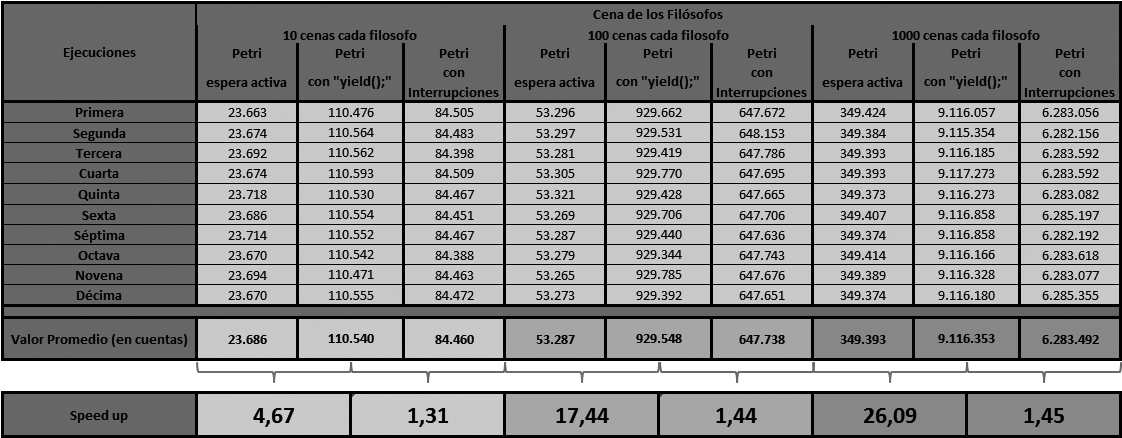
\includegraphics[width=0.9\linewidth,keepaspectratio]{./resultados_conclusiones/resultados/img/resultados38}
			\caption{Tabla comparativa de los distintos m�todos de espera de disparos para el problema de la cena de los fil�sofos}
			\label{fig:resultados38}
		\end{figure}
		
		La tabla de la Figura \ref{fig:resultados38} muestra que, por la raz�n mencionada anteriormente, esperar activamente
		por la ejecuci�n de un disparo es la opci�n m�s r�pida, $4,67$ veces mejor que el uso de la funci�n \emph{yield()} para
		$10$ cenas, $17,44$ veces mejor en $100$ cenas y, cuando se realizan $1000$ cenas es mas de $26$ veces mejor.
		�sto se produce porque el procesador de Redes de Petri es capaz de resolver disparos en \textbf{\emph{2 ciclos}}, por lo
		tanto, puede tener un disparo resuelto mucho antes de que el hilo consulte si ya se ha realizado su ejecuci�n y, dado que
		los fil�sofos pueden comer todas las veces que lo deseen dentro de su franja de tiempo de procesador que el sistema
		operativo le asigna, siempre pueden encontrar que su disparo fue ejecutado. 
		
		Luego, descartando la espera activa que es por mucho el mejor de los escenarios para �ste problema se observa que el uso
		de interrupciones para �ste problema es $1,31$ veces mejor que el uso de la funci�n \emph{yield()} para
		$10$ cenas, $1,44$ veces mejor en $100$ cenas y, cuando se realizan $1000$ cenas es $1,45$ veces m�s r�pido.
		
		La explicaci�n para estos resultados es que la funci�n \emph{yield()} produce un cambio de contexto y el sistema
		operativo asignar� tiempo de procesador a el resto de los hilos antes de volver a asignarlo al hilo que espera la
		ejecuci�n de su disparo. En cambio, al utilizar interrupciones, el hilo se suspende en un sem�foro, como la resoluci�n
		del disparo es muy r�pida en el IP core, se genera la interrupci�n que reactiva al hilo y lo deja proseguir su ejecuci�n.
		Es necesario un cambio de contexto para atender la interrupci�n pero, el hilo puede proseguir despu�s del mismo sin esperar
		al resto.
		
		El c�digo fuente que resuelve le problema de la cena de los fil�sofos sin interrupciones puede ser encontrado en la 
		secci�n \ref{sec:programa_cena_filosofos_petri}, p�gina \pageref{sec:programa_cena_filosofos_petri}. El c�digo que 
		si utiliza interrupciones, est� en la secci�n \ref{sec:programa_cena_filosofos_petri_int}, p�gina 
		\pageref{sec:programa_cena_filosofos_petri_int}.
		
						
	